\documentclass[
  fontsize=12pt,
  paper=a4,
  parskip=half,
  headings=big,
  DIV=12
]{scrreprt}
\usepackage{graphicx}
\graphicspath{{./figures/}}
\usepackage{caption}
\captionsetup{
  skip=5pt,
  font=small,
  labelfont=bf,
  justification=justified,
  width=0.9\textwidth,
  format=plain
}
\usepackage[style=apa, uniquename=false]{biblatex}
\addbibresource{references.bib}
\counterwithout{figure}{chapter}
\counterwithout{table}{chapter}
\counterwithout{equation}{chapter}
\usepackage{nomencl}
\makenomenclature
\usepackage[hidelinks]{hyperref}
\usepackage{tabularx}
\usepackage{booktabs}
\usepackage{rotating}
\usepackage{array}
\usepackage{float}
\usepackage{amsmath}
\usepackage{xurl}
\usepackage{cleveref}
\AtEveryBibitem{\clearfield{eprint}}

\begin{document}

% title page based on this template: https://www.overleaf.com/latex/templates/umea-university-report-template/jrhgwkpppvpy
\begin{titlepage}
    \thispagestyle{empty}
    \begin{large}
        \begin{tabular}{@{}p{\textwidth}@{}}
            \textbf{UNIVERSITY OF LEIPZIG}\\
            \textbf{Institute for Earth System Science and Remote Sensing} \\
            \textbf{Remote Sensing Products for Earth System Research} \\
        \end{tabular}
    \end{large}
    \vspace{25mm}
    \begin{center}
        \vspace{20mm}
        \LARGE{\textbf{Multiple factors drive post-fire vegetation recovery in tropical peat forests \\ A random forest study in Kalimantan, Indonesia}} \\
        \vspace{25mm}
        \begin{normalsize}
            \begin{tabular}{ll}
                \textbf{Authors} & \\[6pt]
                Giovanna Limon \\
                Elsa Neumann \\
                Nina Preu\ss ler \\
                Nurisa Wijayanti \\
            \end{tabular}
        \end{normalsize}
        \vfill
        \normalsize{March 15, 2026}
    \end{center}
\end{titlepage}

\chapter*{Abstract}
%%% Summarize the key aspects of your research, including the objective, methods, results, and conclusions.

Tropical peatlands in Indonesia are increasingly affected by wildfires that cause severe ecological damage and large carbon losses. However, little is known about what factors drive recovery after fire in this ecosystem. This study investigated post-fire vegetation recovery in peatland forests across Kalimantan, Indonesia, after the severe 2015 fire season. Using the Enhanced Vegetation Index (EVI) derived from MODIS satellite data, vegetation recovery rates were calculated for a short-term (2 years) and longer-term period (5 years). Random forest regression was used to evaluate how recovery rates were related to pre-fire vegetation condition, fire history, burn severity, aridity, distance to intact forest, distance to drainage canals, human footprint, and elevation. On average, burned peatland forests had regained about 80\% of their pre-fire EVI values within two years and exceeded them after five years. Model performance was moderate with $R^2 = 0.56 \pm 0.02$ for 2-year recovery and $R^2 = 0.52 \pm 0.02$ for 5-year recovery. The most influential predictors were aridity, distance to drainage canals, and pre-fire EVI, while fire history had surprisingly little predictive power. Higher aridity index values, indicating more humid conditions, were generally associated with better recovery, consistent with the moisture dependence of tropical peatlands, though the relationship was highly non-linear. The high importance of drainage distance (with higher recovery rates closer to canals) may partly reflect restoration interventions rather than a purely hydrological effect. The relatively low importance of fire history for EVI-based recovery contrasts with studies showing its strong influence on species composition, highlighting that spectral indices such as EVI capture canopy greenness but not the ecological quality of recovering vegetation. These findings suggest that post-fire recovery in tropical peatlands is shaped by a combination of climatic, hydrological, and antecedent conditions rather than any single factor. To our knowledge, this represents the first model assessment of post-fire vegetation recovery in tropical peat forests.

\tableofcontents

% list of abbreviations
\nomenclature{\textbf{dNBR}}{Difference Normalized Burn Ratio}
\nomenclature{\textbf{ESA}}{European Space Agency}
\nomenclature{\textbf{EVI}}{Enhanced Vegetation Index}
\nomenclature{\textbf{GLC}}{Global Land Cover}
\nomenclature{\textbf{GEE}}{Google Earth Engine}
\nomenclature{\textbf{MODIS}}{Moderate-resolution Imaging Spectroradiometer}
\nomenclature{\textbf{RF}}{Random forest}
\nomenclature{\textbf{RMSE}}{Root Mean Square Error}
\nomenclature{\textbf{VRR}}{Vegetation Recovery Rate}
\renewcommand{\nomname}{List of abbreviations}
\printnomenclature

\chapter{Introduction}

It is estimated that Indonesia has the largest area of tropical peatlands on the planet. Previous estimations for the total land area are 13.43 million ha in 2021; with exceptional depths of up to 10 m (\cite{anda_revisiting_2021}). The ecosystem services that peatlands provide include soil formation, fresh water supply, fiber and fuel, climate regulation, biodiversity habitats, and erosion protection (\cite{anda_revisiting_2021}, \cite{setiawan_spatio-temporal_2025}). With high productivity rates of 13.2 Mg C ha$^{-1}$ y$^{-1}$, tropical peat forests play a critical role in the carbon cycle and have some of the largest stocks of carbon on Earth, approximately 57 Gt of CO$_2$ (\cite{kauffman_total_2025}).

Peatlands in their natural condition are usually well protected against fires due to their high moisture content (\cite{kiely_new_2019}). However, over the past few decades, large areas of these landscapes have been deforested and drained for agricultural use (\cite{kiely_new_2019}; \cite{schmidt_fire_2024}). These changes lead not only to land subsidence but also to an increased risk of forest fires that are now more frequent, longer in duration, and that penetrate deeper into the peat (\cite{anshari_peatland_2026}; \cite{dadap_drainage_2021}). Many wildfires in Southeast Asia are intentionally set by farmers to clear vegetation for plantations, which are increasingly likely to spread beyond their intended extent (\cite{rein_smouldering_2021}; \cite{schmidt_fire_2024}). However, wildfires can also be caused by natural events, such as lightning (\cite{rein_smouldering_2021}). While in 1997, the largest amount of burned area was measured in primary forests, this changed to plantations and degraded peatlands in 2015 (\cite{setiawan_spatio-temporal_2025}). In the same year, 53\% of the registered fires happened on peatlands, which only constitute up to 12\% of Indonesia’s area (\cite{kiely_new_2019}).

Tropical peatlands burn not only on the surface, but also underground due to smoldering in the peat, which is particularly susceptible to fire due to its high carbon content (\cite{grosvenor_catastrophic_2024}; \cite{rein_smouldering_2021}; \cite{setiawan_spatio-temporal_2025}). While flaming on the surface is characterized by high speed and high temperatures, smouldering is the main combustion process in tropical peatlands, spreading at around 1 cm h$^{-1}$ and having more intense effects on the soil (\cite{rein_smouldering_2021}). This allows the fire to spread further, even after the flaming stopped, and can result in fires that last for several weeks or even years, having continuous negative effects on public health, economy, and climate (\cite{grosvenor_catastrophic_2024}; \cite{kiely_new_2019}; \cite{rein_smouldering_2021}; \cite{schmidt_fire_2024}). While there are attempts to detect smoldering fires using remote sensing, as in \textcite{sofan_detection_2019}, most remote sensing products, and therefore also this study, focus on detecting fires above the ground.

The El Niño-Southern Oscillation (ENSO) is one of the main drivers of variations in the transport of air moisture and ocean surface temperature in and around Indonesia, causing differences in groundwater levels and ultimately fire seasons, typically ranging from August to October (\cite{grosvenor_catastrophic_2024}; \cite{schmidt_fire_2024}). Therefore, intensified El Niño conditions due to climate change and the resulting droughts in the region are responsible for more frequent and more intense fire seasons in the region (\cite{schmidt_fire_2024}; \cite{setiawan_spatio-temporal_2025}). The most destructive fire seasons between 1980 and 2017 occurred in 1982–1983, 1997–1998, 2006, 2009, 2013, and 2015 (\cite{kiely_new_2019}), largely coinciding with known El Niño years (\cite{gan_greenhouse_2023}). This highlights the correlation between the ENSO and wildfires (\cite{schmidt_fire_2024}).

Tropical forests can withstand destruction by wildfires and return to their original state within several years (\cite{harrison_impacts_2024}; \cite{setiawan_spatio-temporal_2025}). However, the recovery of the ecosystem does not always proceed in the same way, but depends on various factors, including the landscape/ecosystem type and its pre-fire condition, landscape heterogenity, tree density, the amount of human intervention, the climate conditions after the fire, the distance to forest areas that remain intact, and, according to \textcite{hoscilo_development_2008} most important, fire frequency and burn severity (\cite{harrison_impacts_2024}; \cite{hoscilo_development_2008}; \cite{schmidt_fire_2024}; \cite{setiawan_spatio-temporal_2025}; \cite{xu_global_2024}). Therefore, the recovery of vegetation depends heavily on local conditions, which vary greatly throughout Indonesia (\cite{setiawan_spatio-temporal_2025}).

Repeatedly burned areas experience stronger biodiversity decline, higher carbon losses, slower recovery, and more simplified vegetation structure. While areas that have been burned once are able to support a multi-layered forest again after recovery, systems that have been burned twice already show a sharp decline or even absence of trees. However, areas that have burned three or even four times do not contain any trunks or trees and show strongly reduced biodiversity, leading to more homogenous landscapes and favoring herbaceous vegetation (\cite{setiawan_spatio-temporal_2025}). These degraded and simplified landscapes are more susceptible to further fire events (\cite{harrison_impacts_2024}; \cite{schmidt_fire_2024}; \cite{setiawan_spatio-temporal_2025}).

In order to effectively support natural recovery after fires, it is essential to understand the temporal dynamics of vegetation recovery and the factors influencing it. While the drivers of post-fire vegetation recovery have been quantitatively analyzed on a global scale (e.g., \cite{xu_global_2024}) as well as in other ecosystems (e.g., \cite{adagbasa_development_2020, joao_indicator-based_2018}), a similar analysis has to date not been conducted for tropical peat forests. Existing studies in these ecosystems have focused on spatial patterns of vegetation recovery (\cite{setiawan_spatio-temporal_2025}) as well as fire effects on ecosystem properties and biodiversity (\cite{harrison_impacts_2024}). The aim of our study is to address this gap by exploring the prediction of post-fire vegetation recovery using a diverse set of factors related to climate, vegetation, hydrology, fire, and more in peat forests in Kalimantan, Indonesia. Specifically, we investigate the following research questions:

- How do different factors influence the short- and longer-term vegetation recovery rates after fires in tropical peat forests?

- How well can random forest regression predict vegetation recovery based on these factors?

To answer these questions, we compute vegetation recovery rates for areas burned in the 2015 wildfire season, which \textcite{grosvenor_catastrophic_2024} described as the worst on record at the time. We then train random forest models to predict recovery rates from a set of eight predictors. By implementing two models -- one for the recovery rate after 2 years and one after 5 years -- we  explore possible differences in the drivers and predictability of short- and longer-term recovery. With this study, we aim to provide a first quantitative estimate of how much and in what way different factors affect vegetation recovery from fires in tropical peat forests and the potential for predicting it.
Thereby, we hope to contribute to a better understanding of post-fire vegetation dynamics in tropical peatlands, enabling more targeted and effective restoration efforts.

\chapter{Methods}
% Detail the research design, and procedures
% Mention software/tools used
% Discuss the data collection and analysis methods

\section{Study area}

Our analysis focused on Kalimantan, the Indonesian part of Borneo Island. Peatlands in this region cover approximately 4.5 million ha ({\cite{anshari_peatland_2026}}). Peat in Kalimantan occurs predominantly in freshwater topogenous peatlands, peat domes, and plain tidal landforms. The depth of the peat is dominated by moderate (100–200 cm) and deep (200–300 cm) classes. A very deep peat ($>$ 700 cm) is found mainly in Central Kalimantan, with smaller occurrences in South Kalimantan (\cite{anda_revisiting_2021}).

Kalimantan has an equatorial tropical climate with high annual rainfall of about 2,500--4,000 mm yr$^{-1}$ (\cite{nurlatifah_drought_2023}). However, a relatively drier season typically occurs in June--September. Fires tend to peak during this period because reduced rainfall lowers peatland water tables, drying the peat and making it more flammable. El Niño events further intensify drought and increase fire occurrence (\cite{schmidt_fire_2024}).

The 2015 fire event, which coincided with the dry season and El~Niño conditions, burned approximately 2.6 million ha across Indonesia, of which about 16\% occurred in Kalimantan, and an estimated 850,000 ha of the burned area was on peatlands \cite{world_bank_group_cost_2016}). These peatland fires were estimated to release $\sim$1.8 Mt C nationally, with Kalimantan contributing 1.02 Mt C ($\sim$3.74 Mt CO\textsubscript{2}) (\cite{setyawati_carbon_2018}).

To identify the specific pixels that would be relevant and suitable for our analysis, we applied a set of five criteria using multiple datasets (Table \ref{tab:data}). The study area selection and all subsequent analyses were conducted in Jupyter Notebooks (where not otherwise specified), relying primarily on the packages rioxarray, xarray (\cite{hoyer_xarray_2017}), numpy (\cite{harris_array_2020}), and matplotlib (\cite{hunter_matplotlib_2007}).

The initial identification of the burned area was based on the MODIS Fire\_cci Burned Area pixel product version 5.1 (FireCCI51), produced by the European Space Agency (ESA) Climate Change Initiative Programme (\cite{chuvieco_esa_2018}), which we retrieved from Google Earth Engine (GEE). This raster data contains burned areas on the day of the year they first burned at a 250 m resolution. We selected only those areas where fires were first detected between August 1 and October 31, 2015 -- the three months in which most fires occurred in 2015 -- and additionally filtered for burned area pixels with a confidence above 40\%. This layer was used as the reference raster to which all other layers were reprojected. From this initial set of pixels, only those classified as peatland as well as forest were kept. To identify the former, we used the Global Peatland Map 2.0, a 1 x 1 km grid provided by the \textcite{greifswald_mire_centre_global_2022}, reprojected using nearest neighbor resampling. Forest was identified based on 30-meter global land cover (GLC) data for 2015 from \textcite{li_improved_2023}, which was reprojected to the target resolution of 250 m using mode resampling. The study area was further reduced to only include pixels that were not converted to cropland by 2021 to ensure that observed changes primarily reflect ecological recovery rather than land-use conversion. For this purpose, we used the 10 m ESA WorldCover 2021 (\cite{zanaga_esa_2022}), which we converted to a cropland binary and then reprojected to 250 m resolution using maximum resampling, so that all pixels that had at least one 10 m pixel with cropland were removed. Lastly, we filtered out pixels where burns occurred again during our study period to avoid confounding effects of repeated burns on the recovery trajectory. This filtering was based on MODIS fire alerts provided by NASA FIRMS. This dataset contains the centroid points of 1 km$^2$ pixels in which a fire is suspected based on brightness, and provides data from 2001 until near-real time. To detect repeatedly burned areas, we applied a 500 m buffer to all fire alerts recorded  after October 2015 that had a confidence of $\geq$ 30\%, and excluded any study area pixel that had at least one intersection with the resulting polygons.

In total, 18326 pixels fulfilled all conditions. This final study area spanned all provinces of Kalimantan, covered a total of 111,600 ha of peatland forest, and clustered in Central and South Kalimantan Province (Fig. \ref{fig:study_area}).

\begin{figure}[H]
    \centering
    \includegraphics[width=\textwidth]{figures/study_area.png}
    \caption{A map showing all of the investigated study sites (marked in red), which are mainly concentrated along the southern coast of the Southeast Asian island of Kalimantan.}
    \label{fig:study_area}
\end{figure}

\section{Vegetation recovery metrics}

The Enhanced Vegetation Index (EVI) was used as a proxy for vegetation in our study. The advantage of the EVI is its increased sensitivity towards high biomass, making it especially suitable for tropical forests as found in Indonesia, where Normalized Difference Vegetation Index (NDVI) values would saturate (\cite{huete_overview_2002}). For example, \textcite{setiawan_spatio-temporal_2025} used the EVI to montitor regrowth trajectories after fires in peatlands in Sumatra, Indonesia.

To quantify the vegetation recovery after fires, we computed the Vegetation Recovery Rate (VRR) using the following formula:

\begin{equation}\label{eq:vrr}
    \text{VRR} = \frac{\text{EVI}_{\text{t}}-\text{EVI}_{\text{post}}}{\text{EVI}_{\text{pre}}-\text{EVI}_{\text{post}}} \cdot 100
\end{equation}

where EVI$_{\text{t}}$ is the EVI at a specified time after the fire, EVI$_{\text{post}}$ is the immediate post-fire EVI, and EVI$_{\text{pre}}$ is the pre-fire EVI. This metric has been used in similar forms to investigate vegetation recovery after fires (e.g., \cite{adagbasa_development_2020}) and earthquakes (e.g., \cite{jiang_evaluating_2015}). We removed pixels in which the difference between pre- and post-fire EVI was below 0.1 since we wanted to predict the vegetation recovery after loss due to fire (Fig. \ref{fig:hist_evi_diff}).

Since we aimed to explore possible temporal differences in how variables influence recovery, we selected two time frames. Short-term recovery was defined as the recovery rate after two years, setting EVI$_{\text{t}}$ to 2017. A longer-term recovery rate was calculated for 2020, five years after the fires.

All EVI layers were based on the MOD13Q1 V6.1 Terra Vegetation Indices (\cite{didan_modisterra_2021}), which provides an EVI band at a 250 m resolution every 16 days. The pre-fire EVI was computed as the 5-year median up until July 31, 2015, and the post-fire EVI as the 3-month median from November 1, 2015, to January 31, 2016. The 2017 and 2020 EVI layers represented yearly medians. The composites were computed and extracted using GEE.

\section{Predictors}

In this section, we detail the eight predictors used in our analysis, both why they were included and how we obtained and processed the data to represent them (Tab. \ref{tab:data}). For an overview of predictor value distributions, refer to Fig. \ref{fig:hist_pred1} and \ref{fig:hist_pred2}.

% table of all raster layers as overview, with name, source...
\begin{sidewaystable}
    \centering
    \caption{Overview of data layers used in this study. All rasters were reprojected to match the Burned Area grid. For references, please refer to the text.}
    \label{tab:data}
    % \begin{tabular}{p{2.5cm} p{3.5cm} p{7cm} p{5cm} p{2cm}}
    \begin{tabular}{>{\raggedright\arraybackslash}p{2.5cm}
                >{\raggedright\arraybackslash}p{3.5cm}
                >{\raggedright\arraybackslash}p{7cm}
                >{\raggedright\arraybackslash}p{5cm}
                >{\raggedright\arraybackslash}p{2cm}}\toprule
          \textbf{Category} & \textbf{Variable} & \textbf{Description}  & \textbf{Data product} & \textbf{Resolution}\\\midrule
          \textbf{Study area} & Burned area & burned pixels between August and October 2015 & MODIS Burned Area (FireCCI51) & 250 m \\
          & Peatland & mask to select peatlands & Global Peatland Map 2.0 & 1 km \\
          & Forest & mask to select forest land cover & GLC-2015 & 30 m \\
          & Cropland 2021 & mask to remove pixels converted to  cropland by 2021 & ESA WorldCover 2021 & 10 m\\
          & Repeated burns & mask to exclude pixels in which another fire occurred after the 2015 fires & MODIS fire alerts & 1 km  \\\midrule
          \textbf{Vegetation recovery} & Pre-fire EVI & 5-year median from August 2010 to July 2015 & MOD13Q1 V6.1 Terra Vegetation Indices & 250 m \\
          & Post-fire EVI & 3-month median from November 2015 to January 2016 & MOD13Q1 V6.1 Terra Vegetation Indices & 250 m \\
          & 2017 EVI & yearly median, used to quantify short-term recovery & MOD13Q1 V6.1 Terra Vegetation Indices &  250 m \\
          & 2020 EVI & yearly median, used to quantify longer-term recovery & MOD13Q1 V6.1 Terra Vegetation Indices & 250 m \\\midrule
          \textbf{Predictors} & Pre-fire EVI & 5-year median from August 2010 to July 2015 & MOD13Q1 V6.1 Terra Vegetation Indices & 250 m  \\
          & Fire history & count of fires between 2001 and 2015 & MODIS fire alerts & 1 km\\
          & Distance to intact forest & distance to forest pixels without burns between 2001 and 2022 & GLC-2015 and MODIS fire alerts & 250 m \\
          & Distance to drainage canals & proxy for water table depth & Drainage canals in Southeast Asia & 5 m \\
          & Burn severity & difference between pre-and post-fire NBR (dNBR) & MOD09A1.061 Terra Surface Reflectance & 500 m  \\
          & Aridity index & & Global Aridity Index & 1 km  \\
          & Human footprint & index of human pressure & Global Human Footprint 2015 & 1 km  \\
          & Elevation & background environmental variable & Global DEM & 250 m  \\\bottomrule
    \end{tabular}
\end{sidewaystable}


\subsection{Pre-fire EVI}

The pre-fire EVI was used as a proxy for biomass before the fire. A similar indicator of pre-fire vegetation was for example used in the global analysis of post-fire vegetation recovery drivers by \textcite{xu_global_2024}, where higher pre-fire productivity was linked to increased recovery times. As mentioned in the previous section, the pre-fire EVI was based on the MOD13Q1 V6.1 product (\cite{didan_modisterra_2021}), summarized as the 5-year median before August 2015 in GEE.

\subsection{Fire history}

Vegetation recovery has been found to take longer and be more heterogenous for forest that has previously burned (\cite{hoscilo_development_2008, setiawan_spatio-temporal_2025}). We therefore included the fire history in the form of a fire count as a predictor layer. We used MODIS fire alerts as a proxy for identifying past fires, the same dataset used to mask out areas that burned again in the study area identification. To count the fires per study area pixel, we applied a 500 m buffer to all fire alerts before August 2015 that had a confidence of $\geq$ 70\%, and calculated the number of intersections each pixel had with the resulting polygons.

\subsection{Distance to intact forests}

Post-fire vegetation recovery in tropical forests is strongly controlled by the availability of seeds for reestablishment (\cite{cury_effects_2020}). Areas that remain unburned can act as so-called fire refugia, which "function as long-term, postfire habitat from which species can expand to neighboring areas, effectively functioning as a seed source" (\cite{meddens_fire_2018}). In a study specifically in Kalimantan, \textcite{hoscilo_development_2008} found the highest above ground biomass after fires in plots close to intact forest fragments. In our analysis, this predictor layer was based on the same forest mask derived from the 2015 land cover data by \textcite{li_improved_2023} previously used to identify the study area. To select intact forest specifically, we filtered out pixels that had burned since 2001 using the fire count layer and that burned again until 2021 using the same mask as for the study area. We then computed a distance raster.

\subsection{Distance to drainage canals}

Drainage canals have been constructed in the majority of Southeast Asian peatlands, where they are used to dry out the organic soil (\cite{dadap_drainage_2021}), thus increasing the water table depth. A study by \textcite{giesen_roles_2023} found that decreasing the water table depth again as part of a peatland rehabilitation project was accompanied by an increase in woody vegetation cover. Because direct data was unavailable, the distance to drainage channels was used as a proxy for water table depth under the assumption that areas close to canals would have lower water tables. A dataset of drainage canals in Southeast Asia by \textcite{dadap_drainage_2021} with a native resolution of 5 m was used for this purpose. Since the computational demand of processing such a high resolution raster was too high for Jupyter notebooks, we conducted the first steps of preprocessing in QGIS. First, the study area raster was vectorized and a 10 km buffer was added to the resulting polygons since the nearest drainage canals might lie outside the study area. Next, we masked the drainage channel raster with the buffered study area. The resulting raster was coarsened to a 50 m resolution using maximum resampling, so that any 50 m containing at least one 5 m pixel with a canal would be marked as canal. This data was then used to compute a distance matrix in Jupyter Notebooks. The final predictor layer was obtained by average resampling to match the reference raster.

\subsection{Burn severity}

While fire intensity describes properties of the fire itself, burn severity refers to the extent of the effects the fire has on the ecosystem (\cite{keeley_fire_2008}). In a modeling study in mountainous grasslands in South Africa, fire severity was one of the most important predictors of ecosystem response-ability after fires (\cite{adagbasa_development_2020}). In the tropical peatlands of Kalimantan, a study on post-fire vegetation succession found the lowest biomass values on plots with the highest burn severities (\cite{hoscilo_development_2008}). We used the Difference Normalized Burn Ratio (dNBR) to quantify burn severity, which describes the difference between the pre- and post-fire NBR:

\begin{equation} \label{eq:dnbr}
    \text{dNBR} = \text{NBR}_{\text{pre}} - \text{NBR}_{\text{post}}
\end{equation}

The NBR values were calculated as:

\begin{equation} \label{eq:nbr}
    \text{NBR} = \frac{\text{NIR} - \text{SWIR}}{\text{NIR} + \text{SWIR}}
\end{equation}

where NIR is the near infrared and SWIR is the short wave infrared surface reflectance band. The data for these bands was obtained from the MOD09A1.061 Terra Surface Reflectance product (\cite{vermote_modisterra_2025}), retrieved via GEE. The layers originally had a resolution of 500 m, but were reprojected to the 250 m reference grid using bilinear resampling.

\subsection{Aridity index}

The aridity index -- calculated as the ratio of precipitation to potential evapotranspiration -- was included to account for possible climatic effects. In their global analysis, \textcite{xu_global_2024} found that aridity affected which factors controlled local recovery times. We used a global aridity index map from \textcite{zomer_version_2022}, reprojecting the 30 arc-second resolution (approximately 1 km) to the reference grid using bilinear resampling.

\subsection{Human footprint}

The Human Footprint was included to explore a possible effect of human pressure on natural vegetation recovery, as \textcite{xu_global_2024} did for their global analysis of drivers of vegetation recovery times. We used a global human footprint map for the year 2015 at a 1 km resolution from \textcite{mu_global_2022}, which was reprojected to 250 m with bilinear resampling. In this dataset, the human footprint falls into a range between 0 and 50, where values up to 4 indicate wild or intact ecosystems, while higher values indicate increasing modification. The score takes into account features such as built environments, population density, and roads.

\subsection{Elevation}

While likely not a direct driver of vegetation recovery, elevation is often included as a background environmental variable when modeling vegetation recovery (e.g., \cite{xu_global_2024, adagbasa_development_2020}). We used a global Digital Elevation Model at a resolution of 250 m from \textcite{hengl_global_2018}, which we aligned with the reference grid using bilinear resampling.

\section{Random forest}

We used random forest (RF) regression to investigate the relationship between vegetation recovery and our chosen predictors. The advantages of this machine learning approach are that it can capture nonlinear relationships as well as variable interactions. It is a frequently used method to predict post-fire vegetation recovery and quantify its drivers (e.g., \cite{xu_global_2024, adagbasa_development_2020, joao_indicator-based_2018}). RF regression was implemented using the scikit-learn package (\cite{pedregosa_scikit-learn_2011}).

To compare predictive power and variable effects between different time frames, we set up separate models with the 2-year and 5-year recovery rate as target variables, respectively. Of the 18326 pixels identified as study area, 13981 had data for all predictor layers and could be used for training and validating the model.

The model performance was evaluated using 10-fold cross-validation. In this approach, the data are randomly split into 10 equal fractions ("folds"). A model is then trained on 9 folds while the remaining fold is used for validation. This process is repeated for each fold, providing a robust measure of model performance with unseen data. The metrics used for evaluating model performance were the coefficient of determination (R$^2$) and the root mean square error (RMSE).

After the cross-validation, a RF model was fitted to the complete data for each target variable. This model was used to evaluate permutation and impurity variable importance, as well as to  explore variable effects on predicted recovery using partial dependence plots.


\chapter{Results}

\section{Vegetation recovery rate}

Within two years, pixels in our study area had regained on average more than 80\% of the EVI lost during the 2015 fires (Fig. \ref{fig:hist_vrr}). Within 5 years, more than 50\% of pixels had recovered completely, with a considerable fraction having a substantially higher EVI in 2020 compared to the pre-fire median (recovery rate $>$ 100\%). The recovery rates for both time frames were roughly normally distributed, with similar standard deviations of approximately $\pm$ 25\%. Short-term recovery rates ranged from -75.1 to 250.42\% while the longer-term recovery had values between -55.98 to 272.05\%.

\begin{figure}[H]
    \centering
    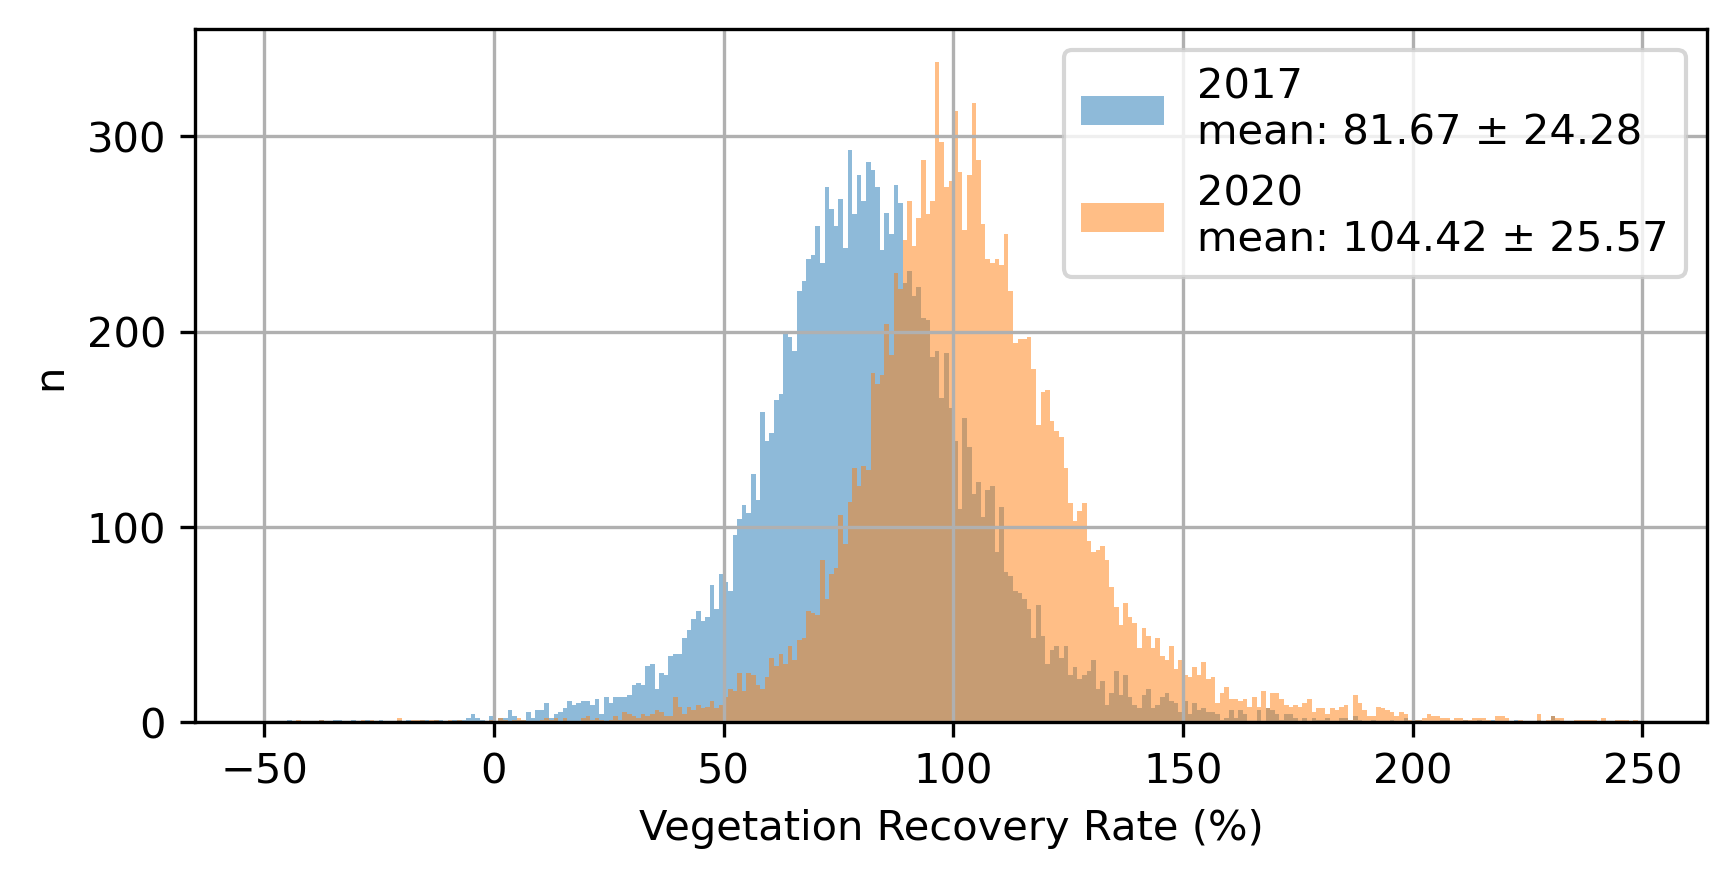
\includegraphics[width=\textwidth]{figures/hist_recovery_rates.png}
    \caption{Distribution of short- (2017) and longer-term (2020) vegetation recovery rates after the 2015 fires. n represents the number of 250 by 250 m pixels in our study area.}
    \label{fig:hist_vrr}
\end{figure}


\section{Random forest model performance}

The random forest models predicted short-term and longer-term vegetation recovery rates moderately well with the chosen predictors (see Table \ref{tab:model_performance}). The amount of variance explained (R$^2$) was slightly higher and the error (RMSE) slightly lower for the short-term recovery prediction. Low standard deviations for all models and metrics indicated stable performance across the 10 training folds.

% table of mean and SD model performance metrics: R2, RMSE, r
\begin{table}[H]
    \centering
\caption{Accuracy and error metrics of random forest models. Both predictor variables are in \%, see Eq. \ref{eq:vrr} for formula. Values indicate mean and standard deviation of values obtained via 10-fold cross-validation.}
\label{tab:model_performance}
    \begin{tabular}{cccc}\toprule
         \textbf{Predicted variable} &  \textbf{R$^2$} &  \textbf{RMSE}\\\midrule
         Short-term vegetation recovery rate (2 years) & 0.56 $\pm$ 0.02  & 16.07 $\pm$ 0.54  \\
         Longer-term vegetation recovery rate (5 years) & 0.52 $\pm$ 0.02  & 17.69 $\pm$ 0.42   \\ \bottomrule
    \end{tabular}
\end{table}

The models for both time frames tended to overestimate low and underestimate high recovery rates (Fig. \ref{fig:obs_pred}). With a bias of -0.14, longer-term recovery was more systematically overestimated than short-term recovery (bias $<$ -0.01).

\begin{figure}[H]
    \centering
    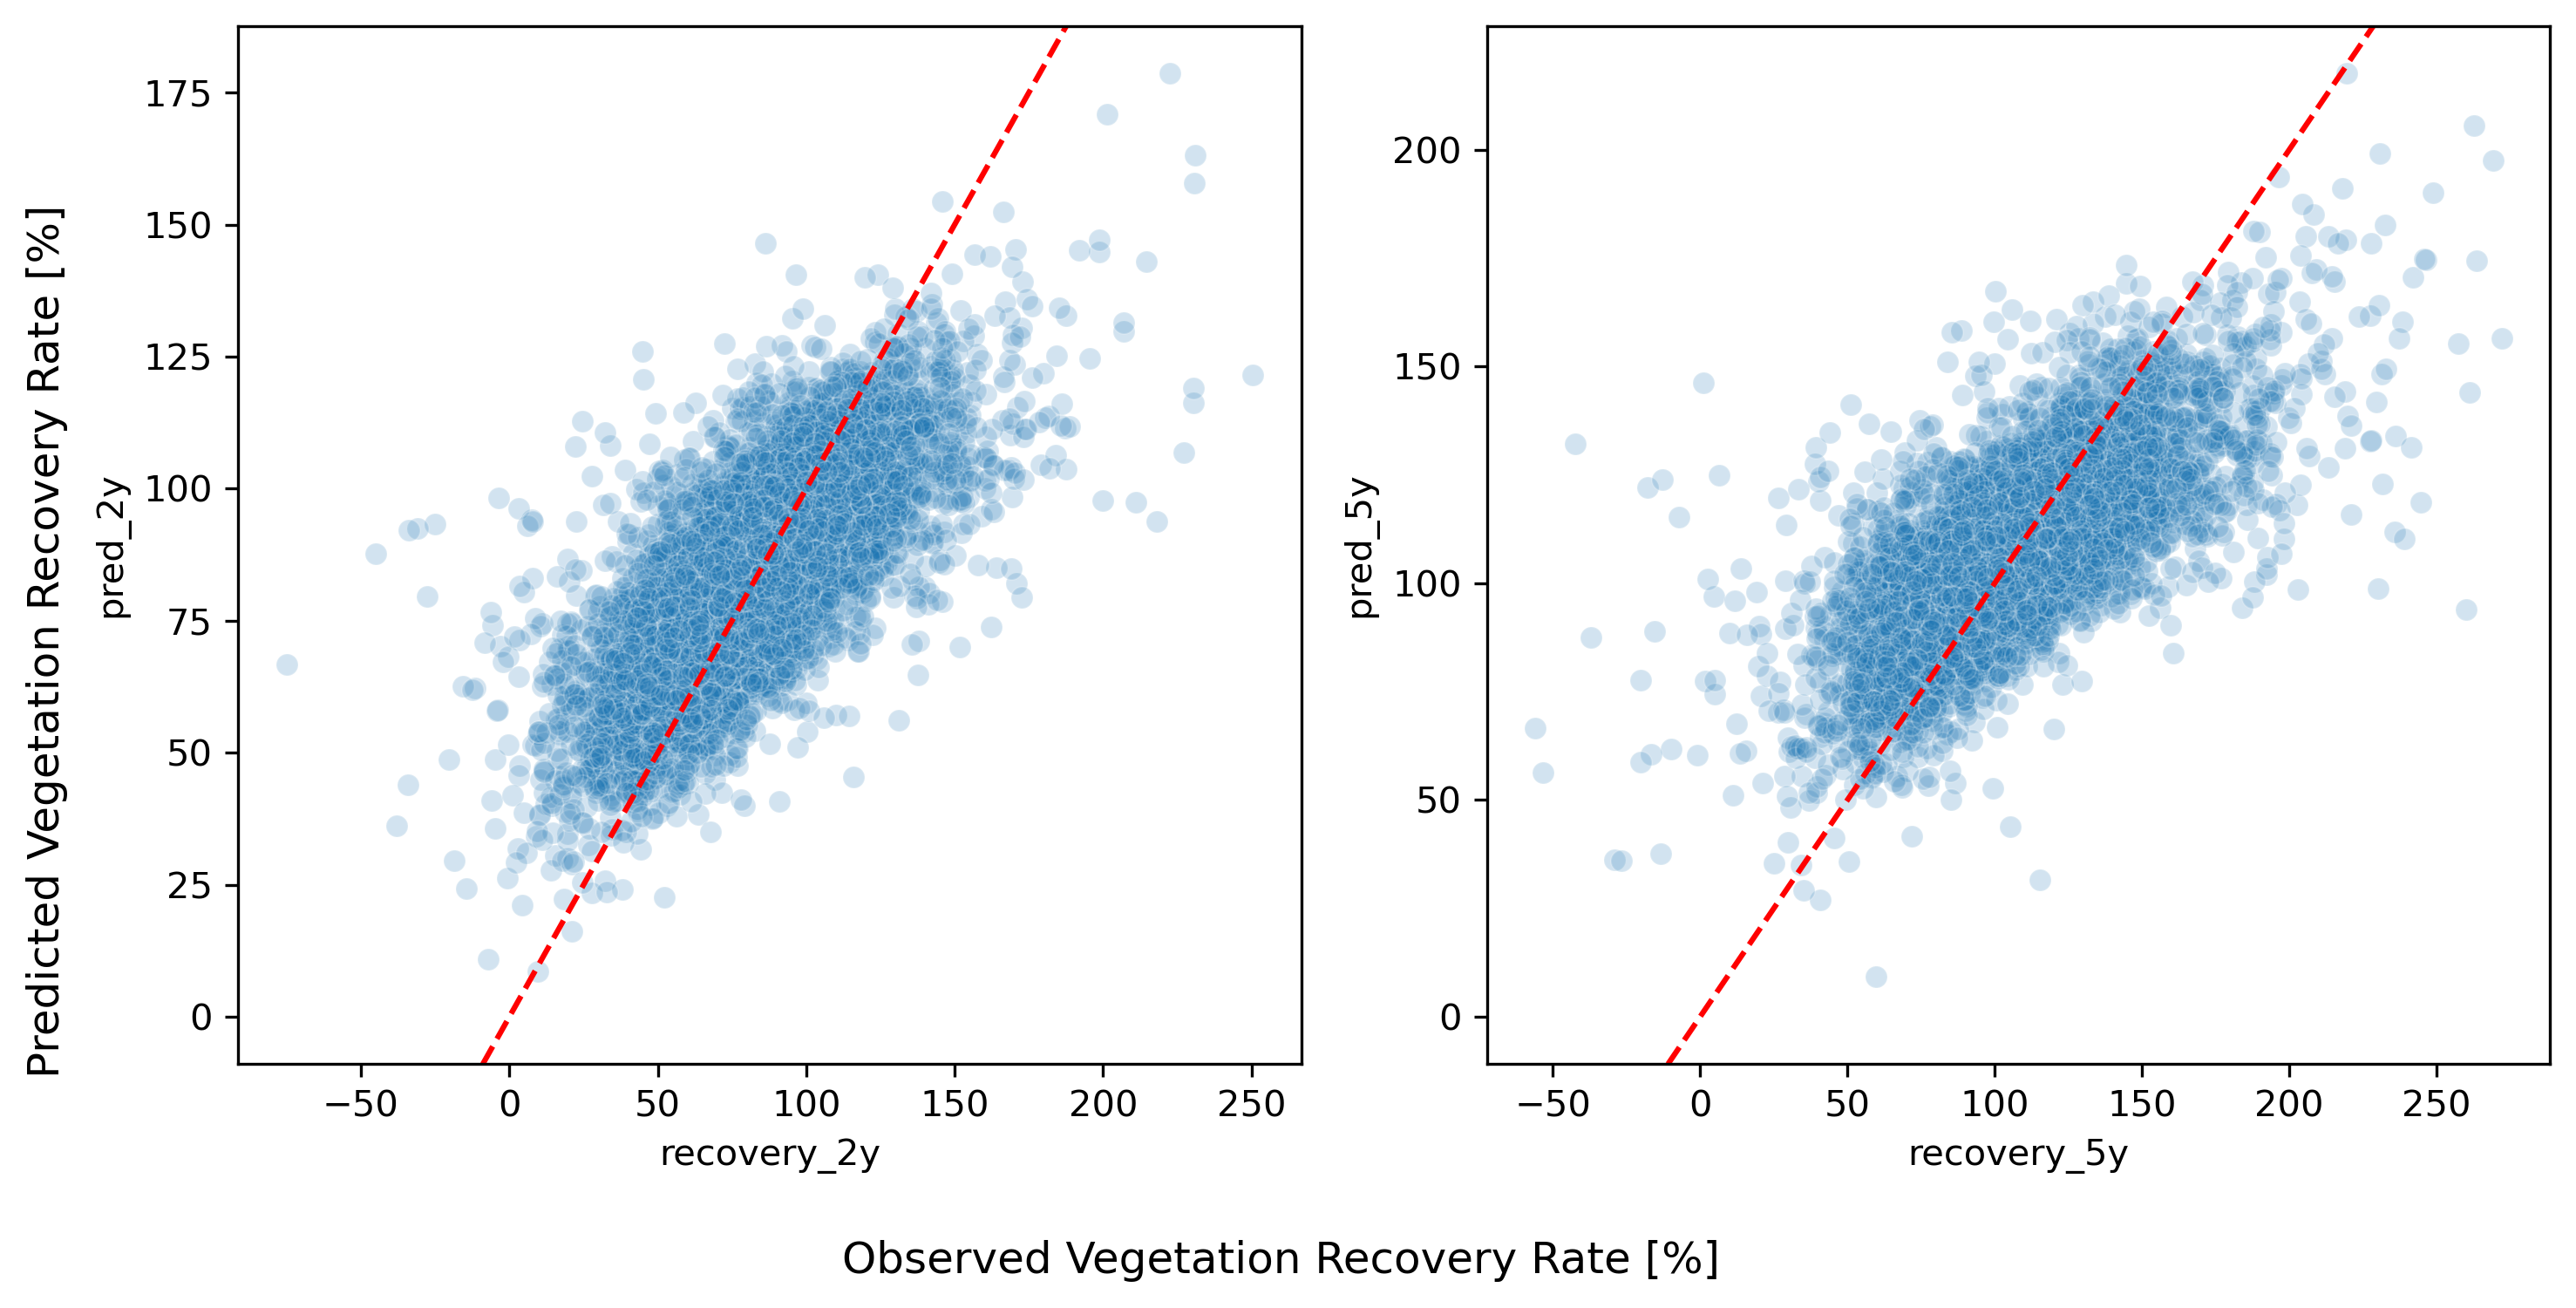
\includegraphics[width=\textwidth]{figures/obs-vs-pred.png}
    \caption{Observed vs. predicted values for the vegetation recovery rate. Colors indicate density of study area pixels per plotted pixel on a log scale. Dashed line represents perfect agreement (observed = predicted).}
    \label{fig:obs_pred}
\end{figure}

\section{Variable importance}

% \begin{figure}[H]
%     \centering
%     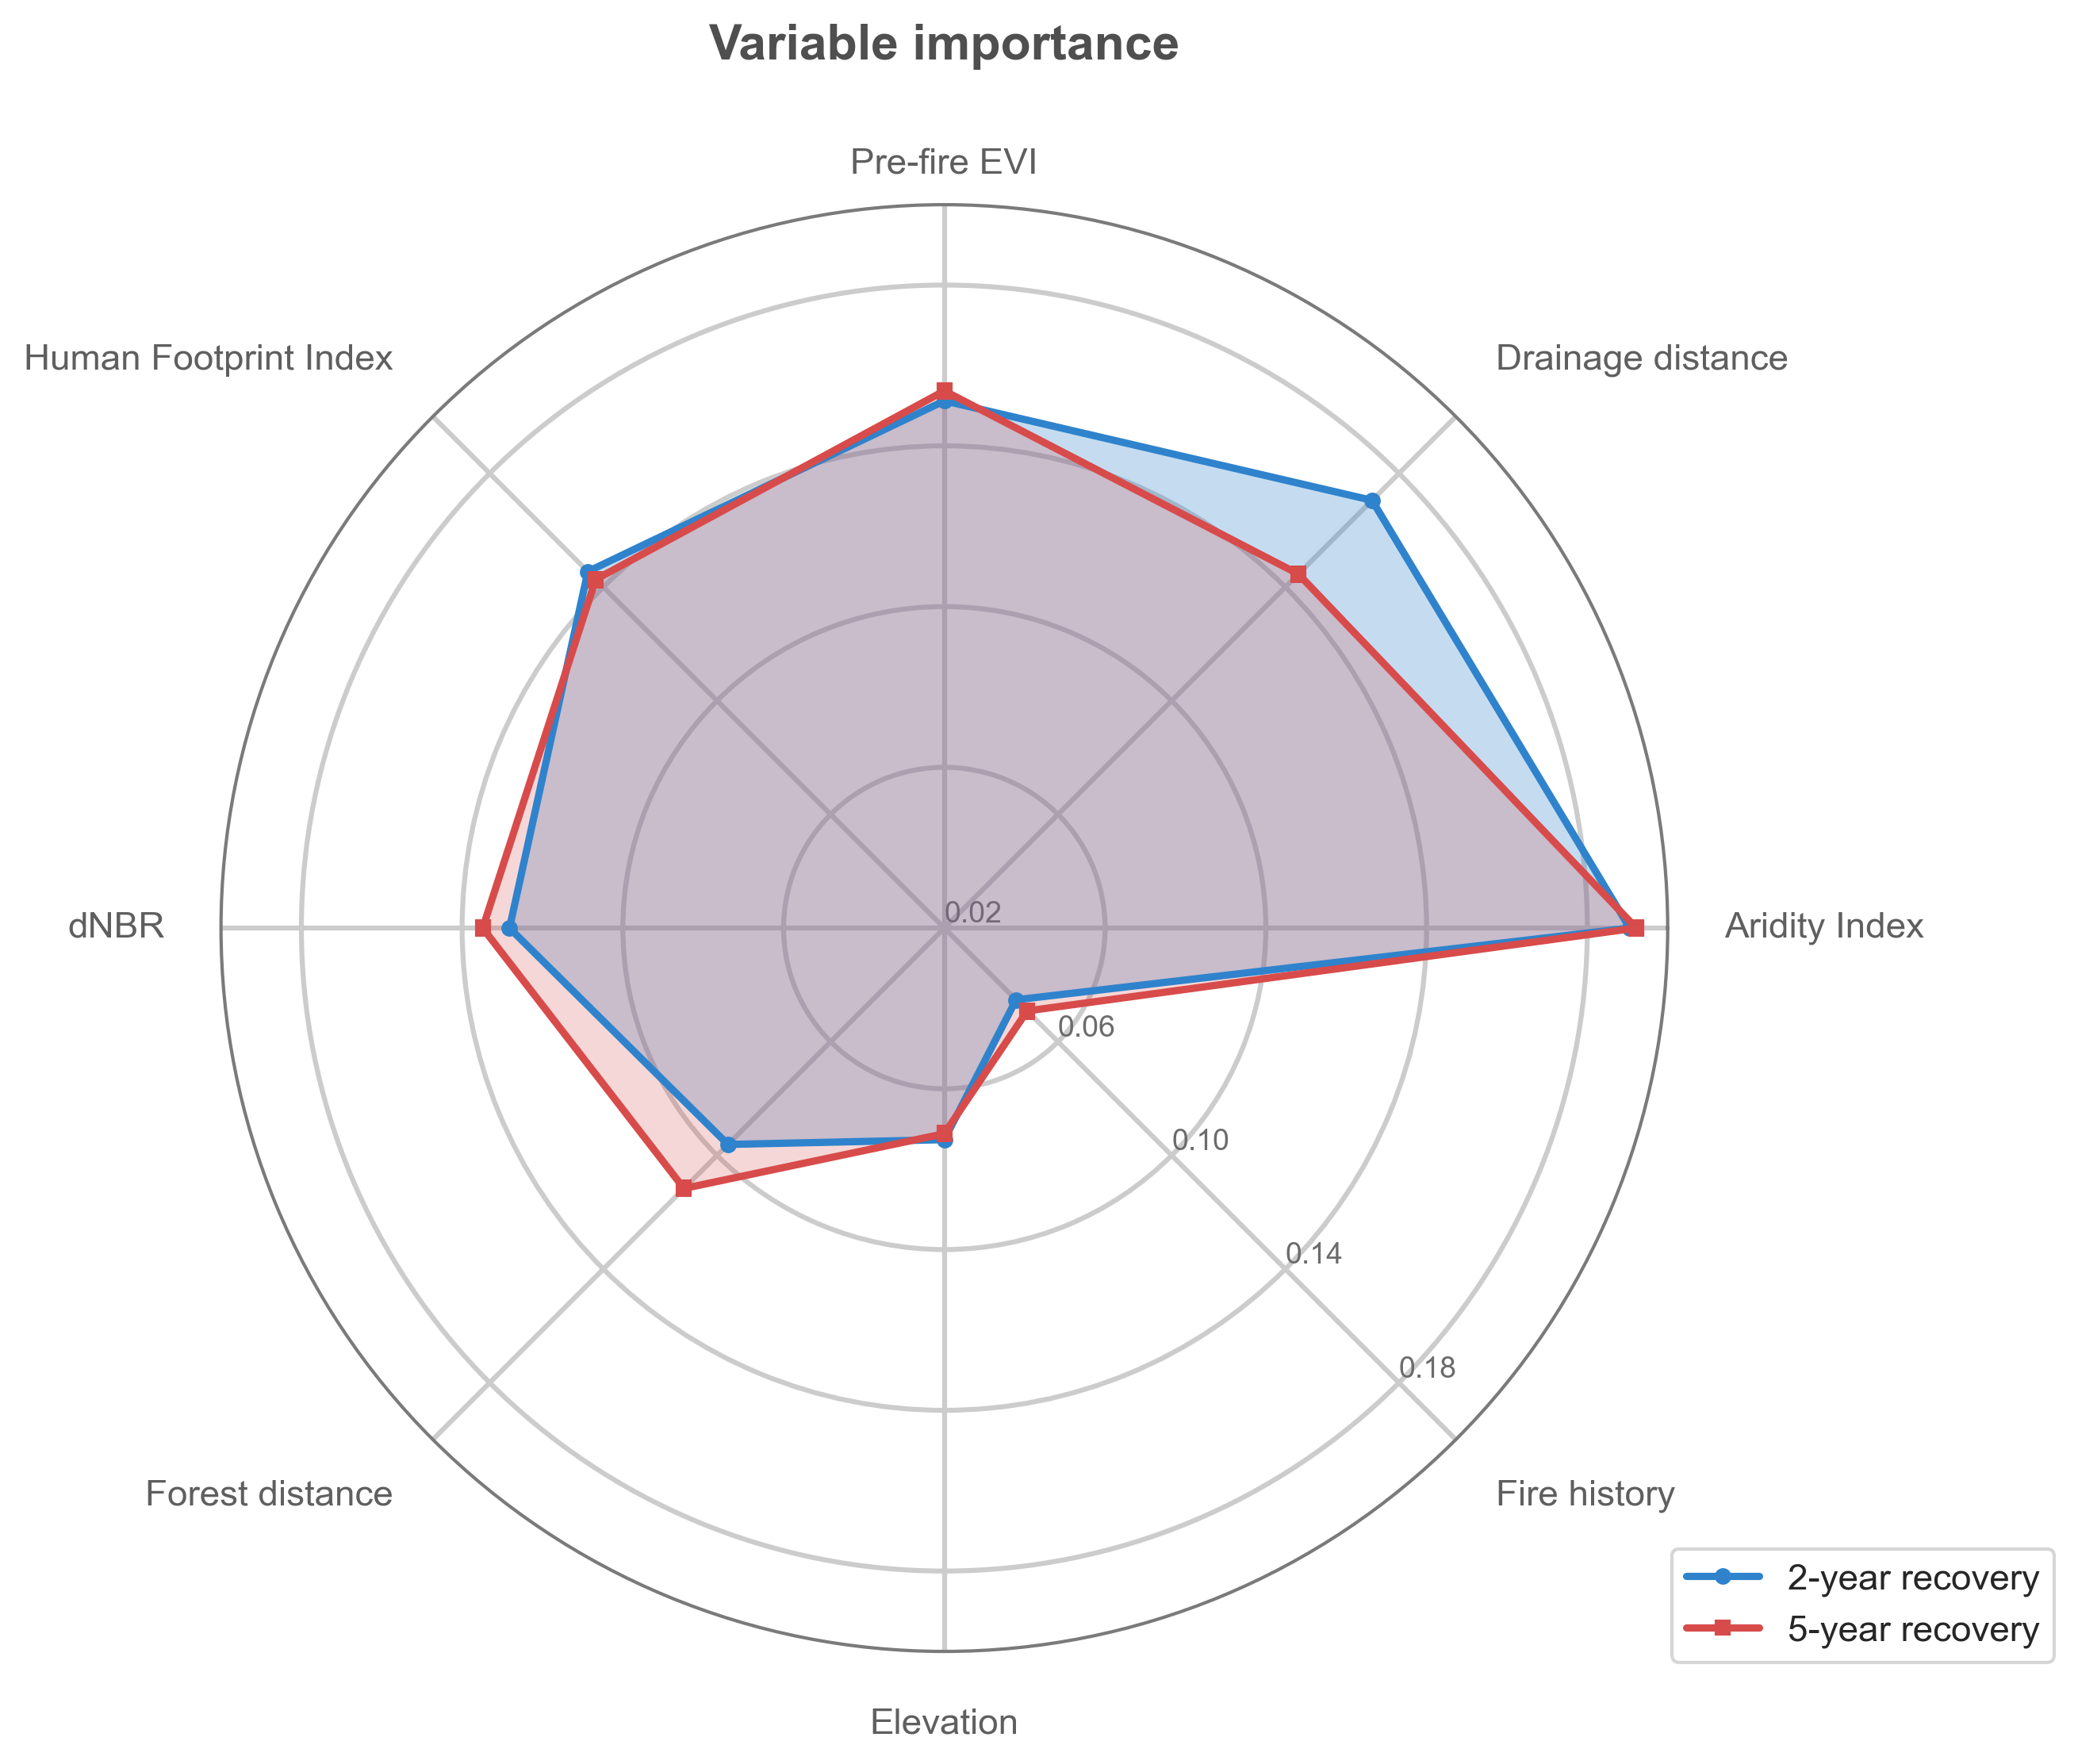
\includegraphics[width=\textwidth]{variable_importance.png}
%     \caption{Variable importance scores from RF models predicting 2-year (blue) and 5-year (red) post-fire vegetation recovery in Kalimantan
%     peatlands. Aridity Index and Pre-fire EVI are the dominant predictors for
%     both time steps, together explaining the largest proportion of variance in
%     recovery rates. Drainage distance is notably more important for 2-year
%     recovery than 5-year recovery, suggesting that water table proximity plays
%     a stronger role in early post-fire regeneration. Fire history shows moderate
%     importance at both time steps, while dNBR (fire severity), Forest distance,
%     Elevation, and Human Footprint Index contribute comparatively less.}
%     \label{fig:var_importance}
% \end{figure}

Most of the included factors were at least moderately important for the prediction of recovery rates (Fig. \ref{fig:perm_imp}). The top five predictors were the same for the short- and longer-term recovery, but in a partly different order. Ranked first for the 2-year recovery was the drainage distance, while pre-fire EVI, aridity index, and the human footprint had only slightly lower values. For 5-year recovery, aridity index was ranked first and had a substantially higher difference to the next-ranked variable than observed anywhere else. The three subsequent variables -- drainage distance, human footprint, and pre-fire EVI -- had very similar importance scores. What both 2-year and 5-year recovery prediction had in common was that fire history was ranked last.

\begin{figure}[H]
    \centering
    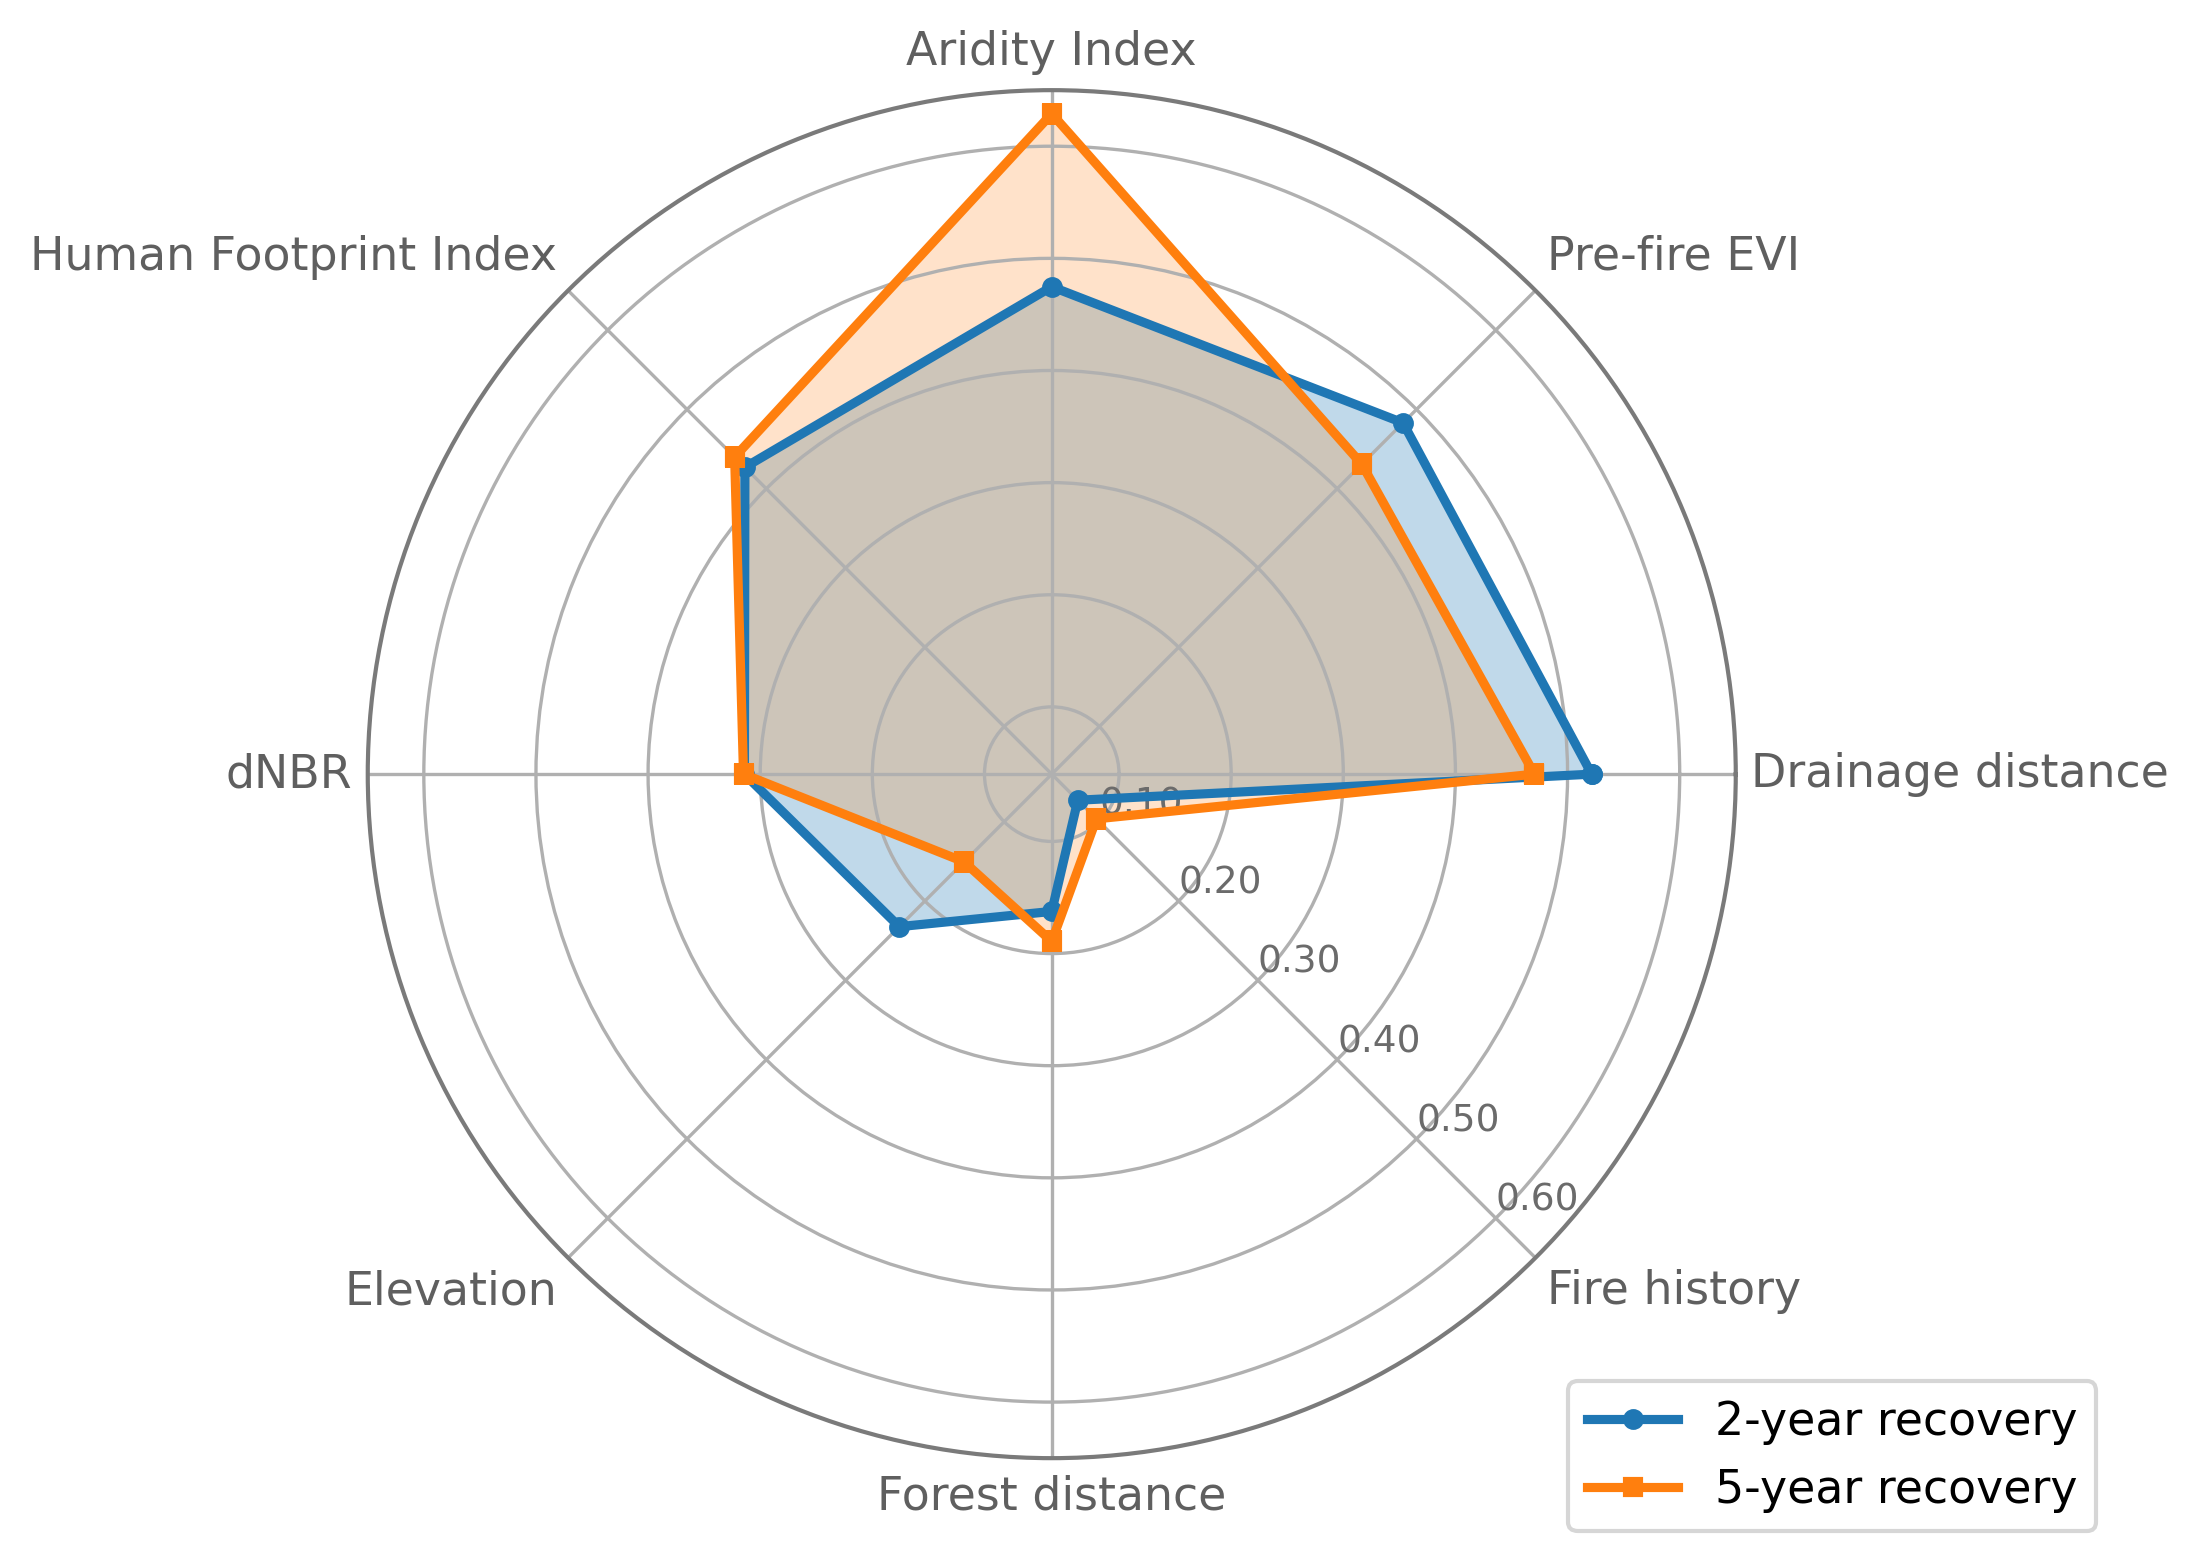
\includegraphics[width=\textwidth]{figures/perm_imp.png}
    \caption{Permutation variable importance. Indicates variable importance for prediction. Computed from random forest models fitted on complete data.}
    \label{fig:perm_imp}
\end{figure}

The impurity importance ranking was more similar between the two predicted recovery rates (Fig. \ref{fig:impurity_imp}). For both, aridity index had the highest importance score, while the scores dropped incrementally for the five subsequent variables. Only the ranking between drainage distance and pre-fire EVI was switched between the two models. As observed for permutation importance, fire count was ranked last in both models.

\begin{figure}[H]
    \centering
    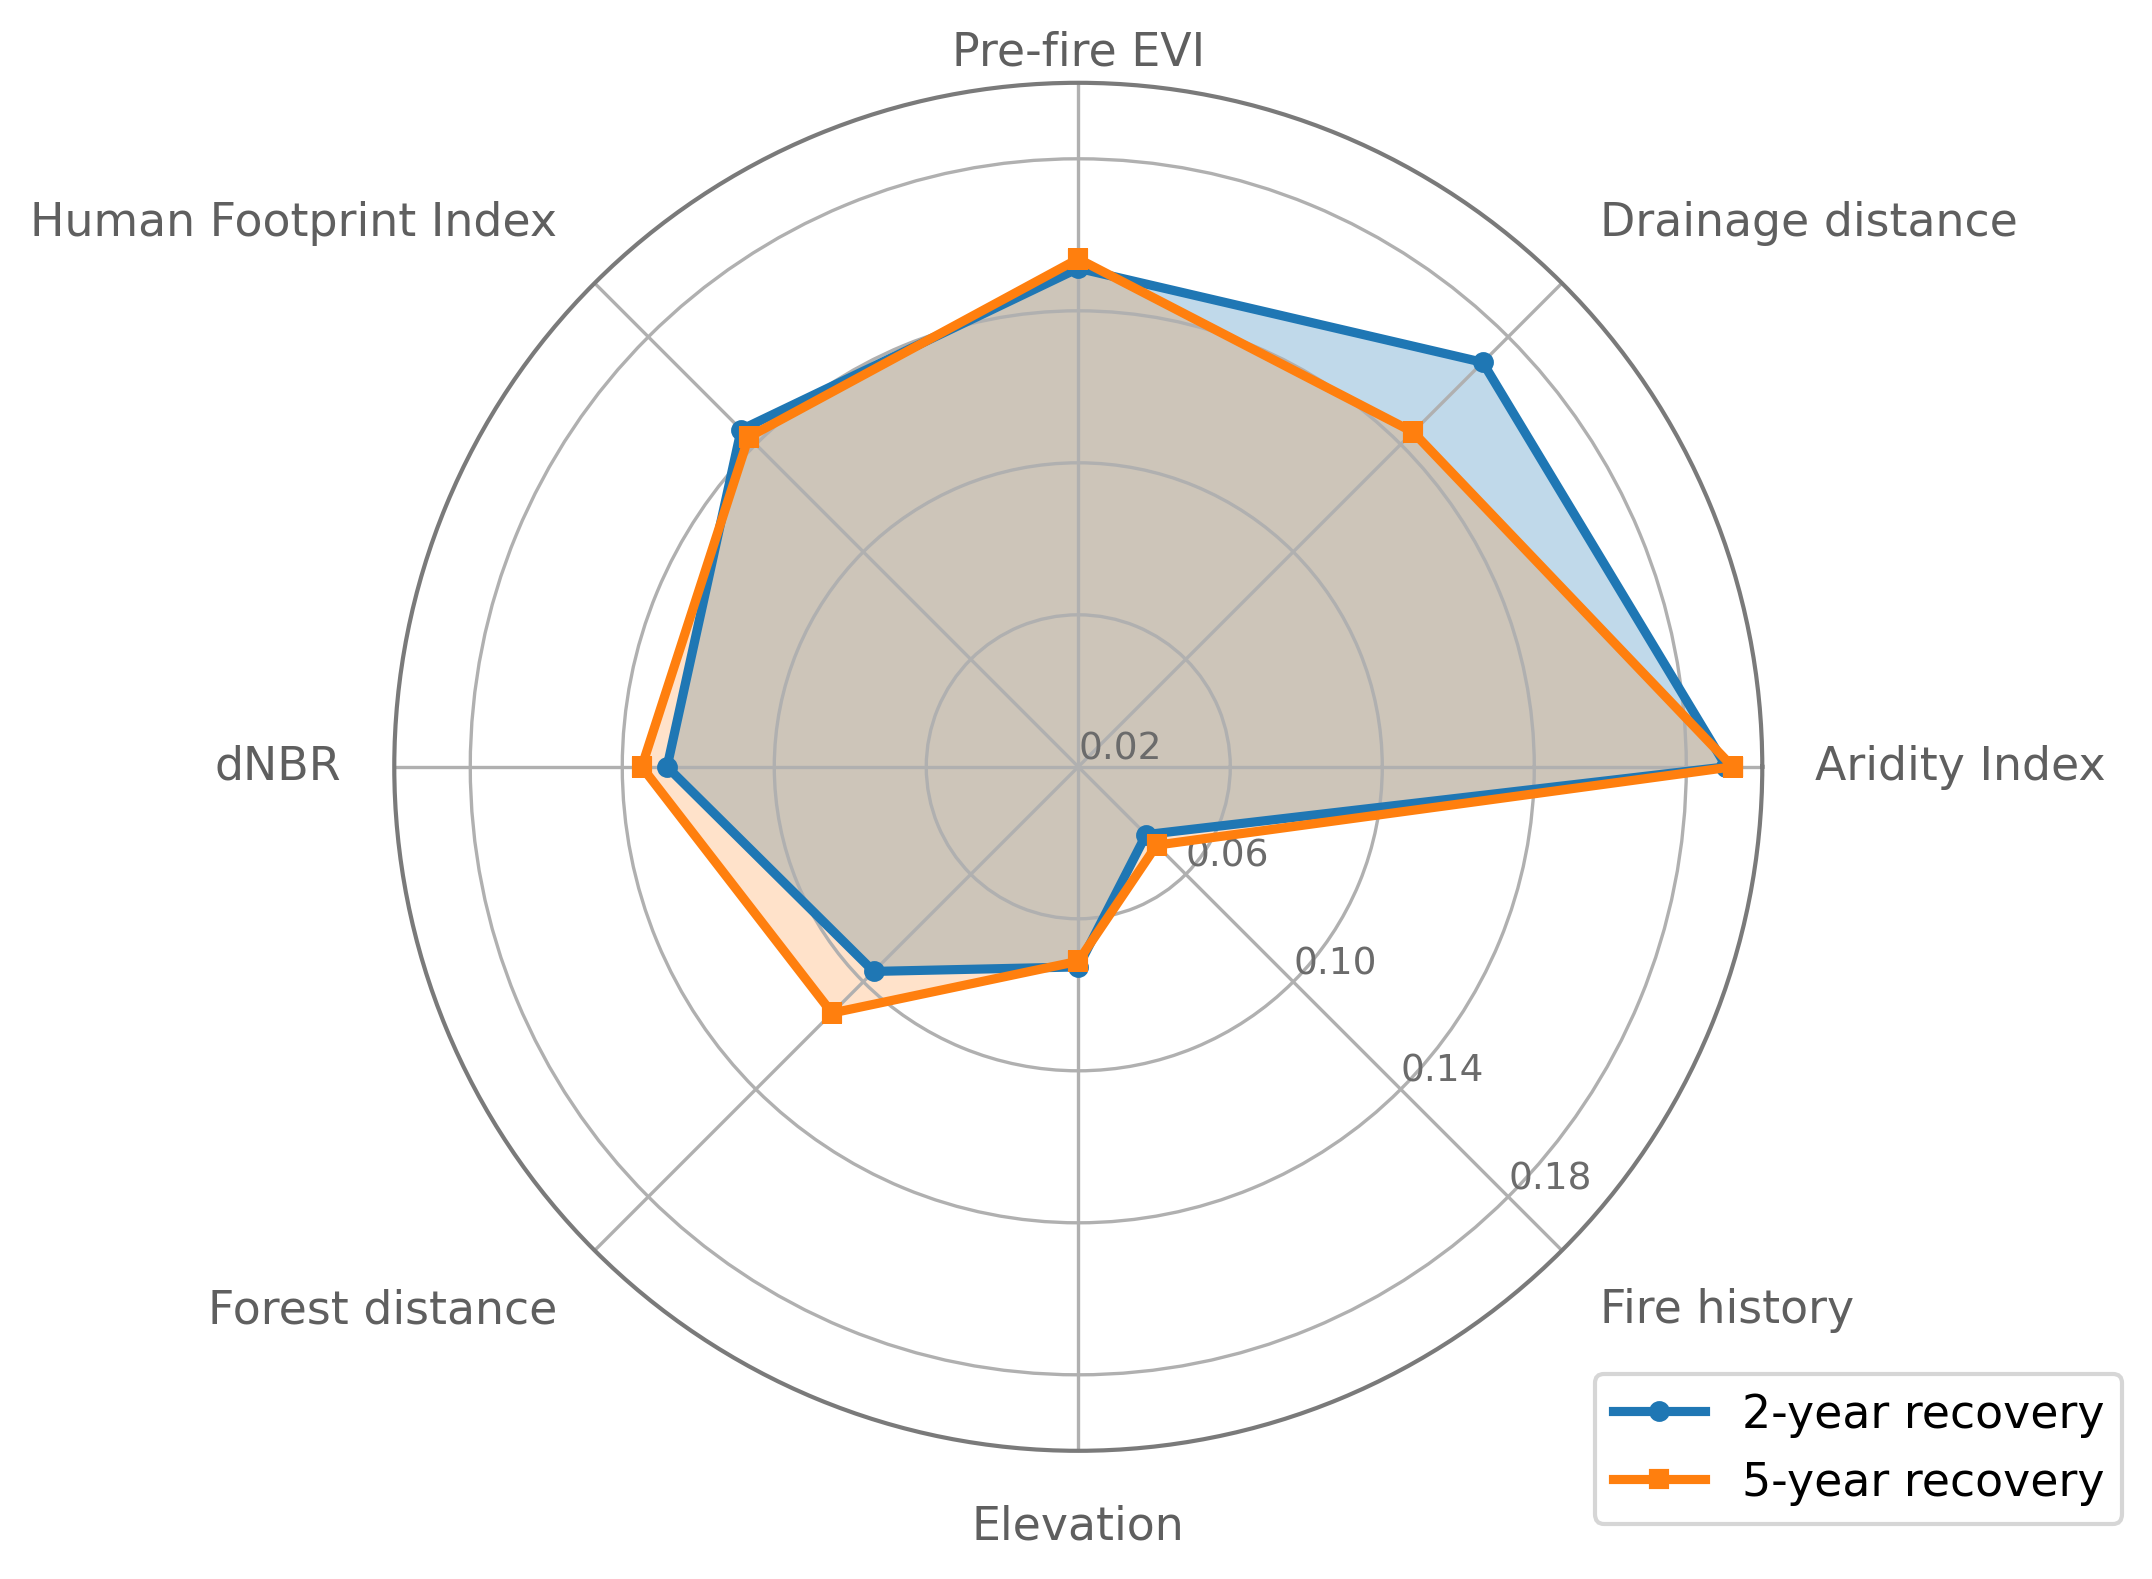
\includegraphics[width=\textwidth]{figures/impurity_imp.png}
    \caption{Variable importance based on mean decrease in impurity. Indicates variable importance during training. Computed from random forest models fitted on complete data. Note the different order of variables compared to Fig. \ref{fig:perm_imp}.}
    \label{fig:impurity_imp}
\end{figure}

\section{Variable effects}

The different factors affected the predicted recovery rates in distinct ways, but with mostly similar effects in the short and longer term (Fig. \ref{fig:pdp_2y} and \ref{fig:pdp_5y}). The pre-fire EVI had the most linear effect, with higher pre-fire medians being associated with lower predicted recovery rates. The aridity index showed a highly non-linear effect on predicted vegetation recovery, with multiple local minima and maxima. Highest predicted recovery rates were associated with the highest and lowest values of the aridity index found in study area pixels (1.7 and 1.9, respectively). Distance to drainage had a strongly negative exponential pattern, where the highest recovery rates were associated with low distance to channels for both time frames. The distance to intact forest had a marginally negative effect of recovery rates. Higher human footprint values -- up to a score of approximately 12 -- were equally associated with higher predicted recovery. Past fire count, when considered in the range of 0 to approximately 7 (the range most study area pixels fell into, see Fig. \ref{fig:hist_pred1}), had a weak negative effect on recovery rates. At higher values, which only very few pixels had, there was no noticeable effect.
The burn severity in the form of the dNBR had a noticeably different pattern in how it affected 2- and 5-year recovery rate prediction. In the short term, predicted recovery rates increased with increasing dNBR. In the longer term, lower recovery rates were predicted for moderate burn severities while both low and high severity led to higher predicted rates. Elevation did not have a straightforward pattern. For the 2-year recovery (where this variable had a slightly higher importance, see Fig. \ref{fig:perm_imp}), highest predicted rates were associated with elevations around 0 and 20 m.

\begin{figure}[H]
    \centering
    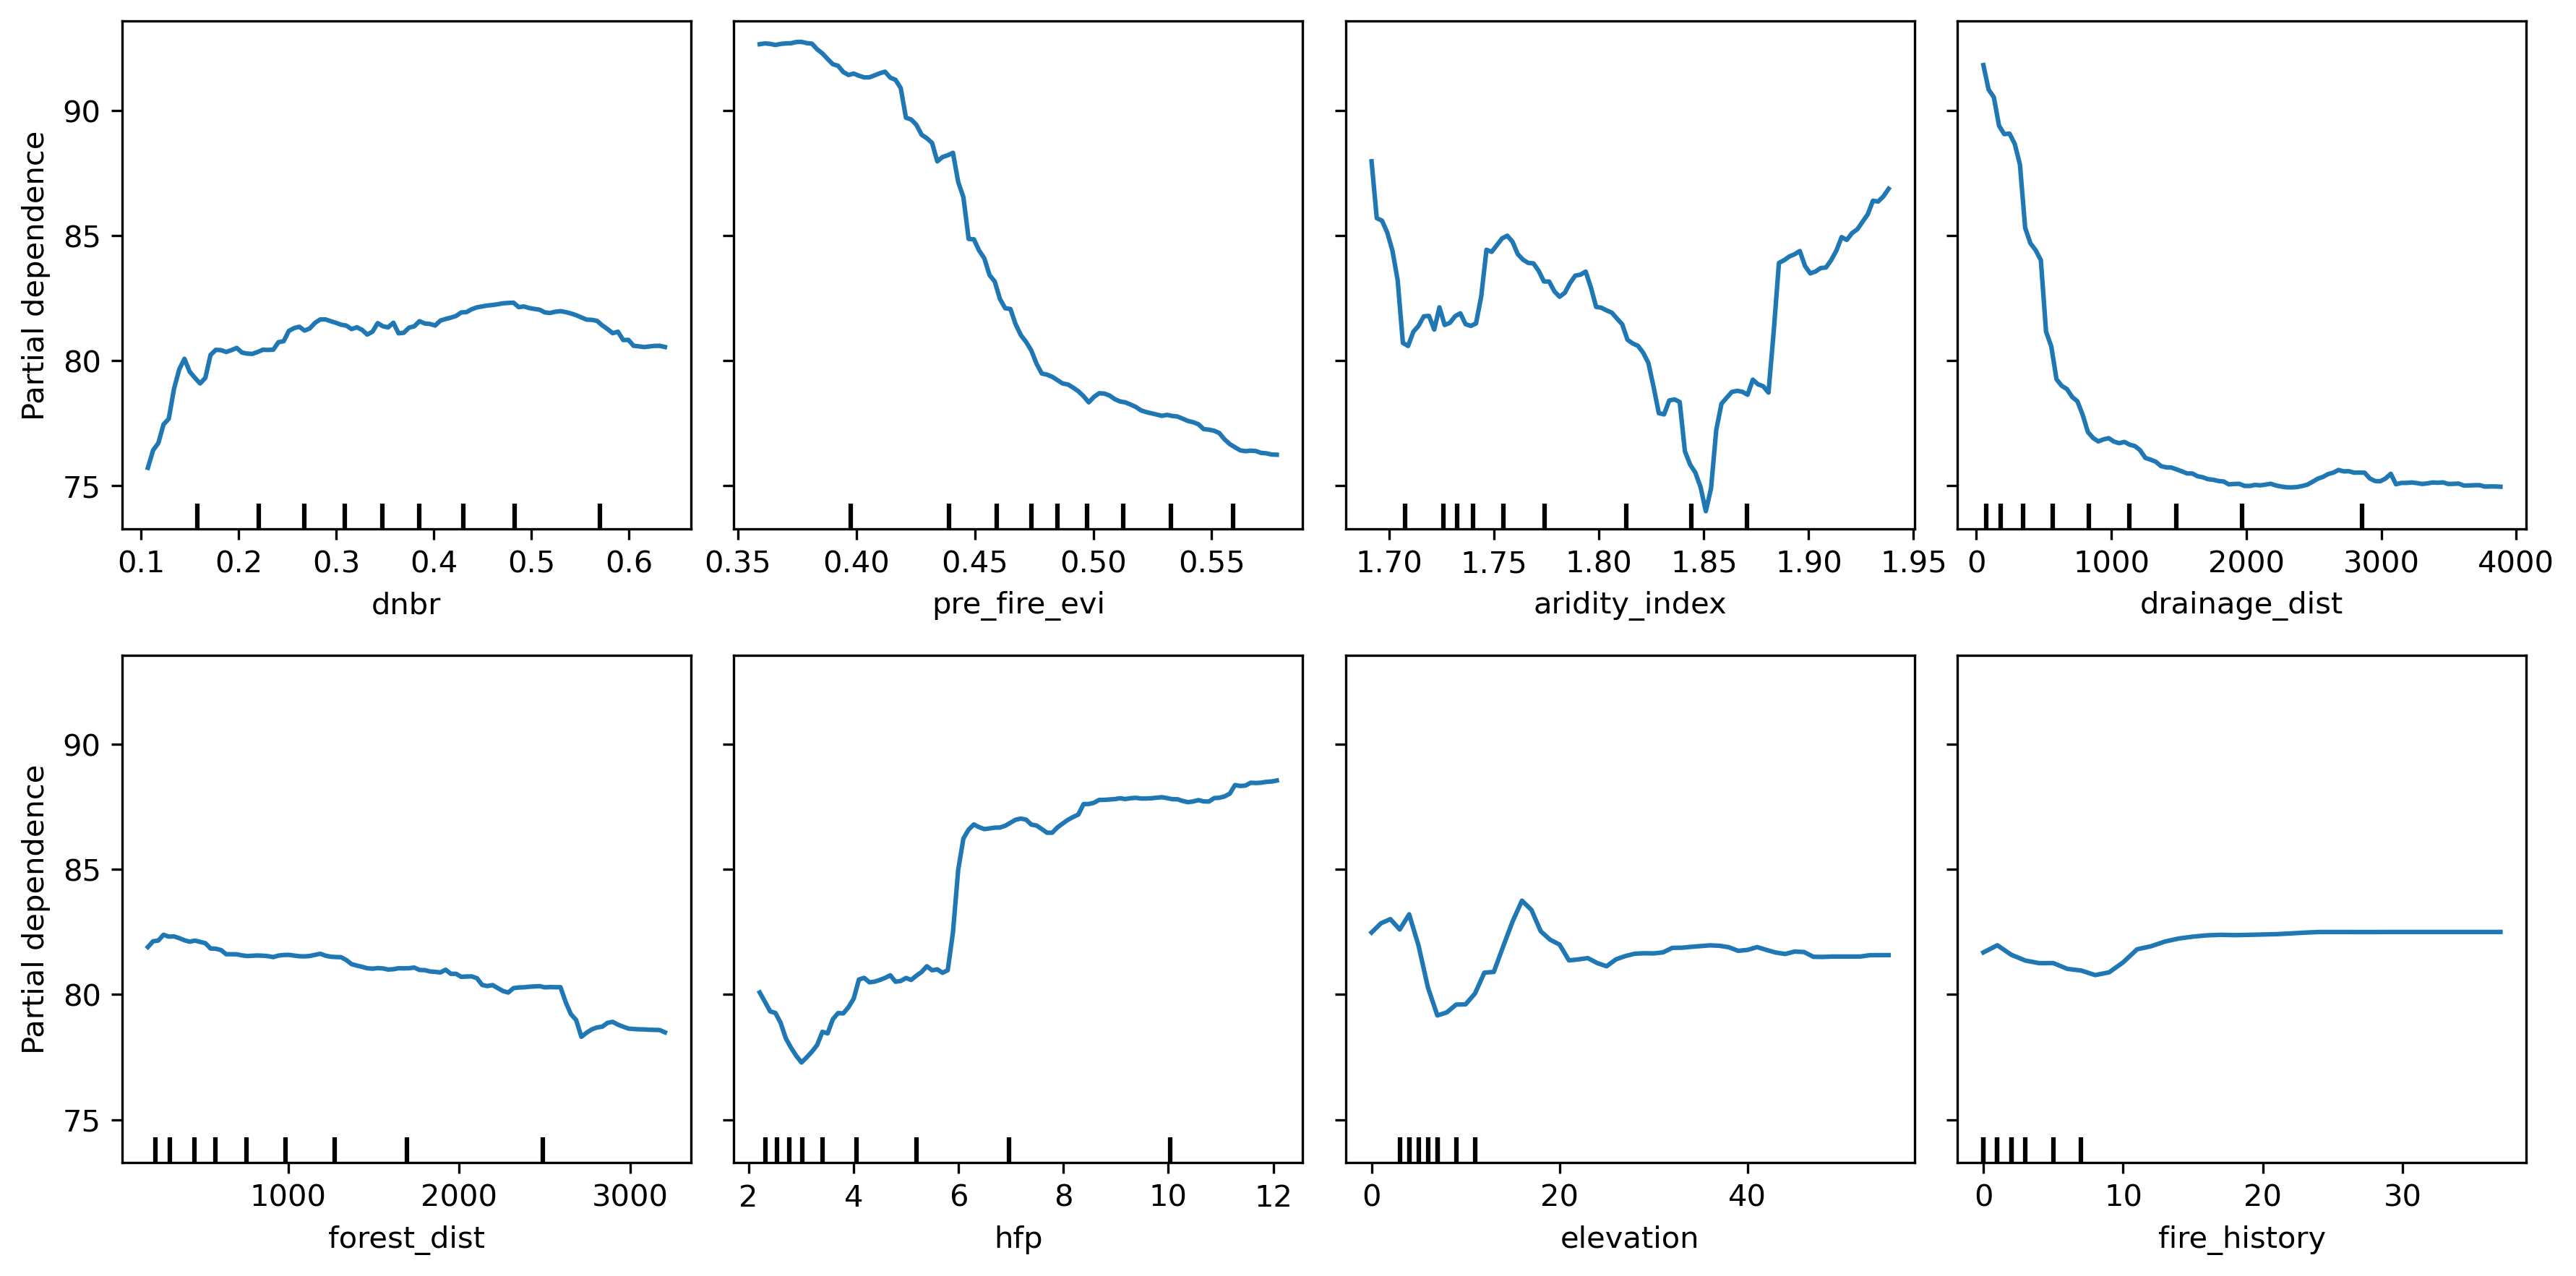
\includegraphics[width=\textwidth]{figures/pdp_2y.png}
    \caption{Partial dependence plots for 2-year recovery rate prediction.}
    \label{fig:pdp_2y}
\end{figure}

\begin{figure}[H]
    \centering
    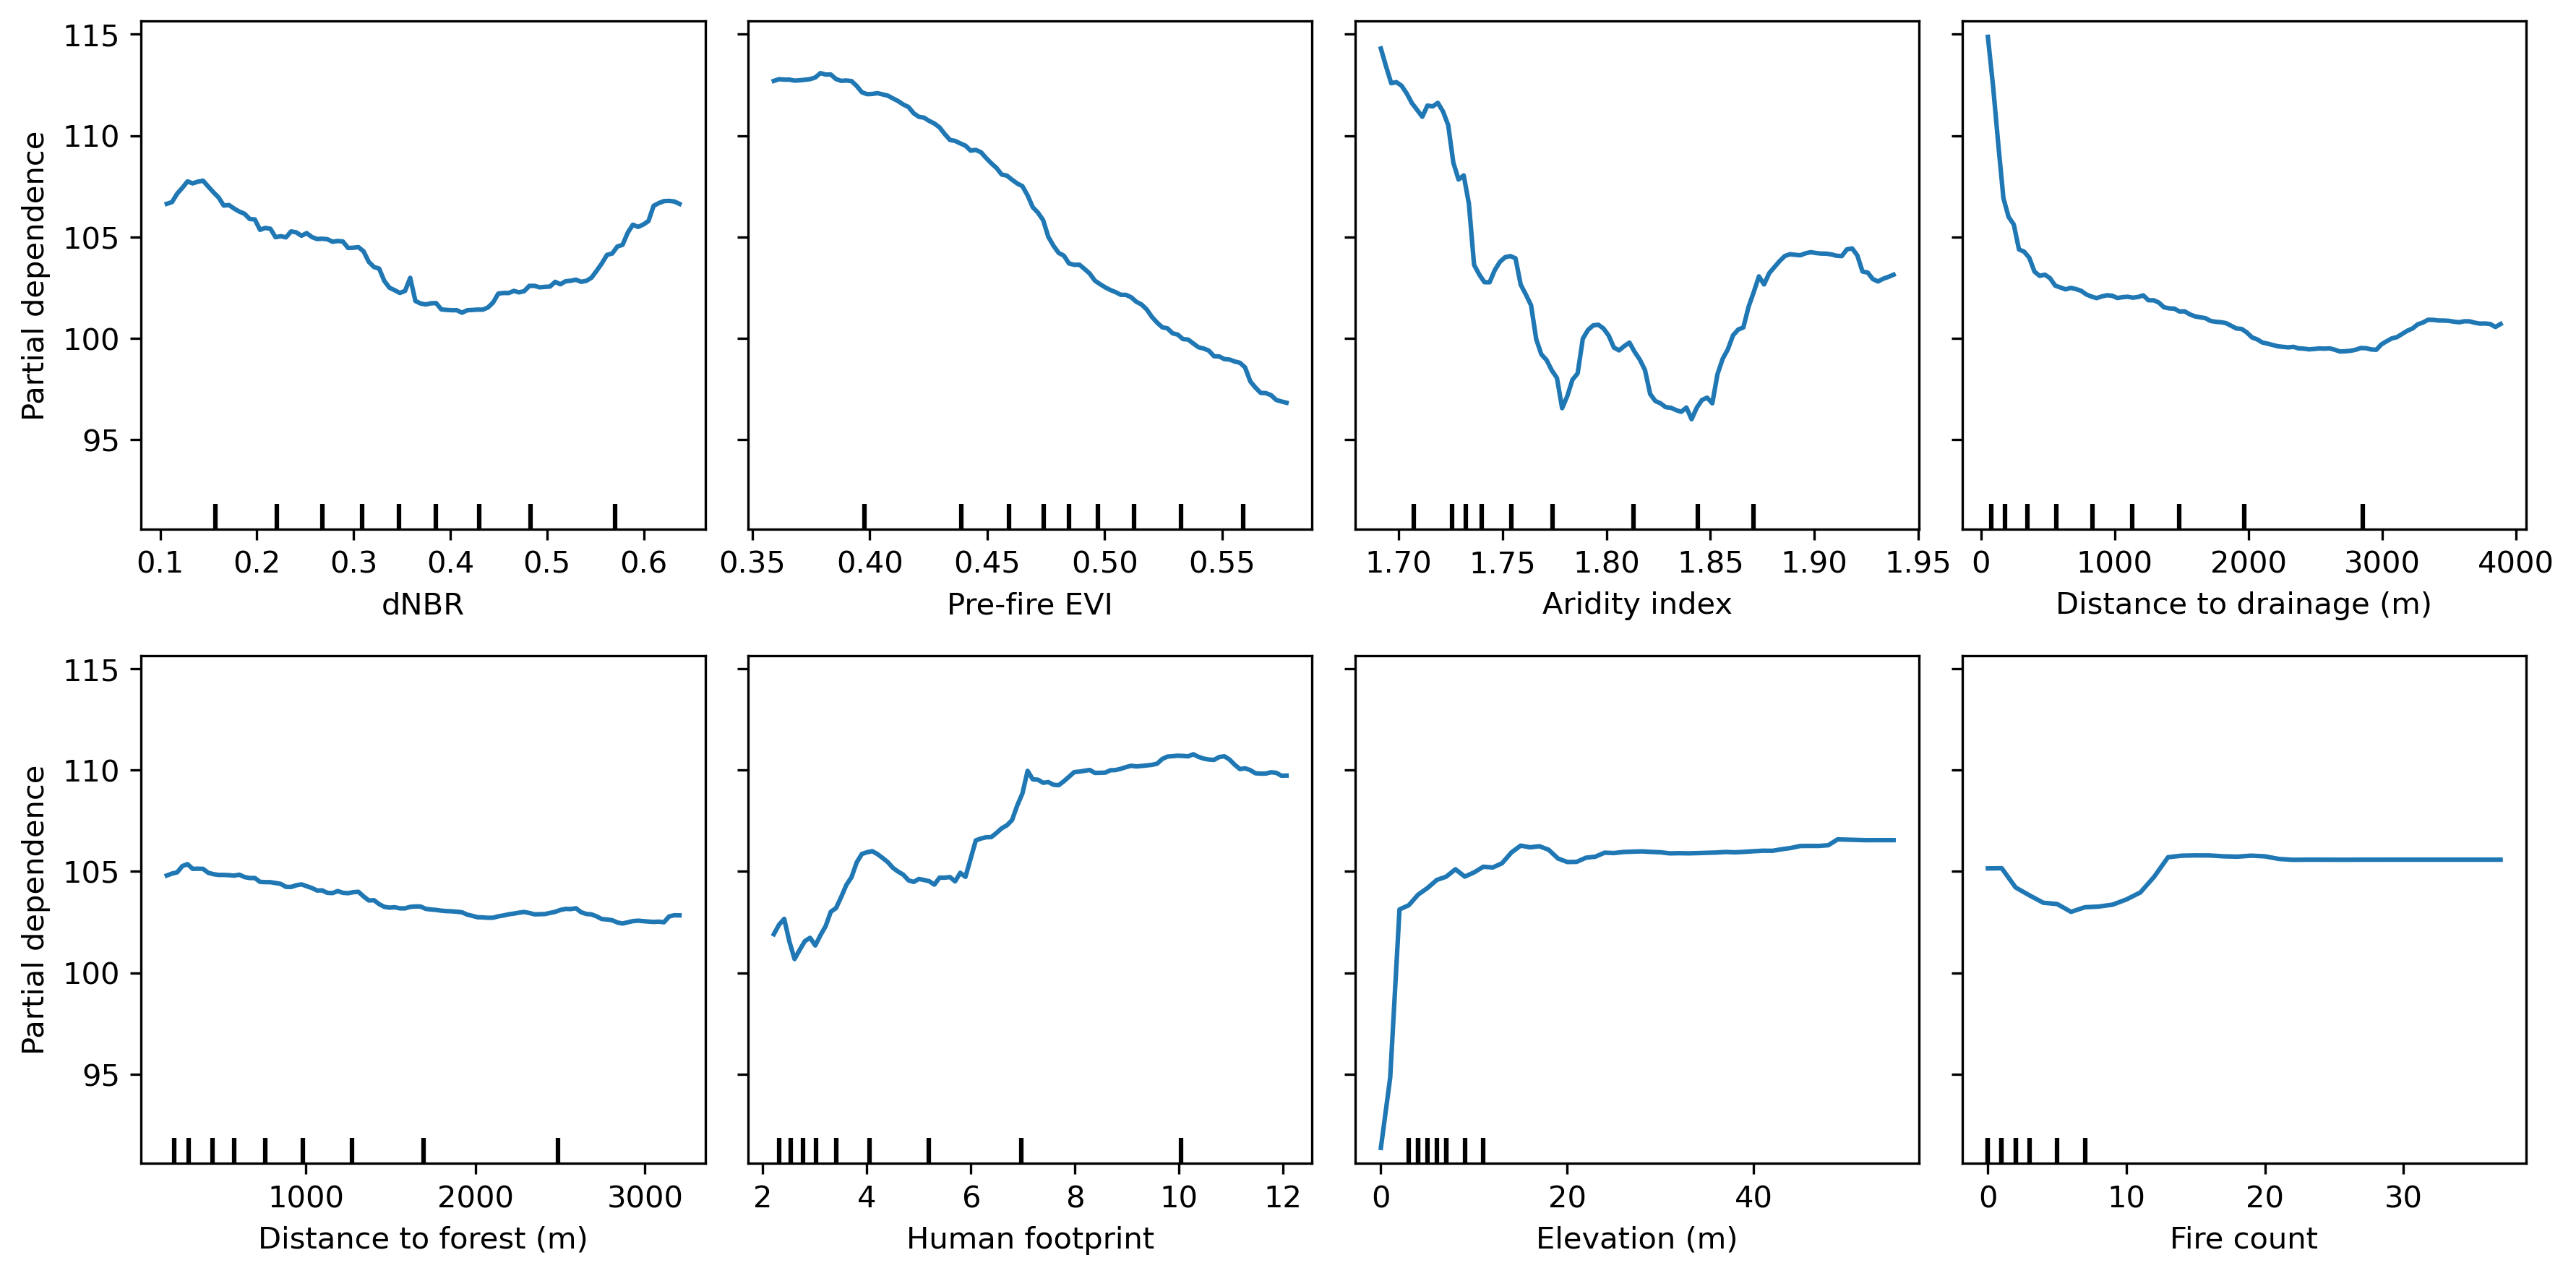
\includegraphics[width=\textwidth]{figures/pdp_5y.png}
    \caption{Partial dependence plots for 5-year recovery rate prediction.}
    \label{fig:pdp_5y}
\end{figure}

Even though they were not the most important variables in the ranking, dNBR and pre-fire EVI showed an interesting interaction (Fig. \ref{fig:pdp_2d}). The highest recovery rates were associated with low pre-fire EVI and low burn severity (bottom left corner). For the short-term recovery, at high pre-fire EVI, the predicted recovery rates were controlled by dNBR, with the lowest rates occurring at low burn severities. In the longer term, however, the lowest recovery rates occurred at the highest pre-fire EVIs, regardless of the dNBR value.

\begin{figure}[H]
    \centering
    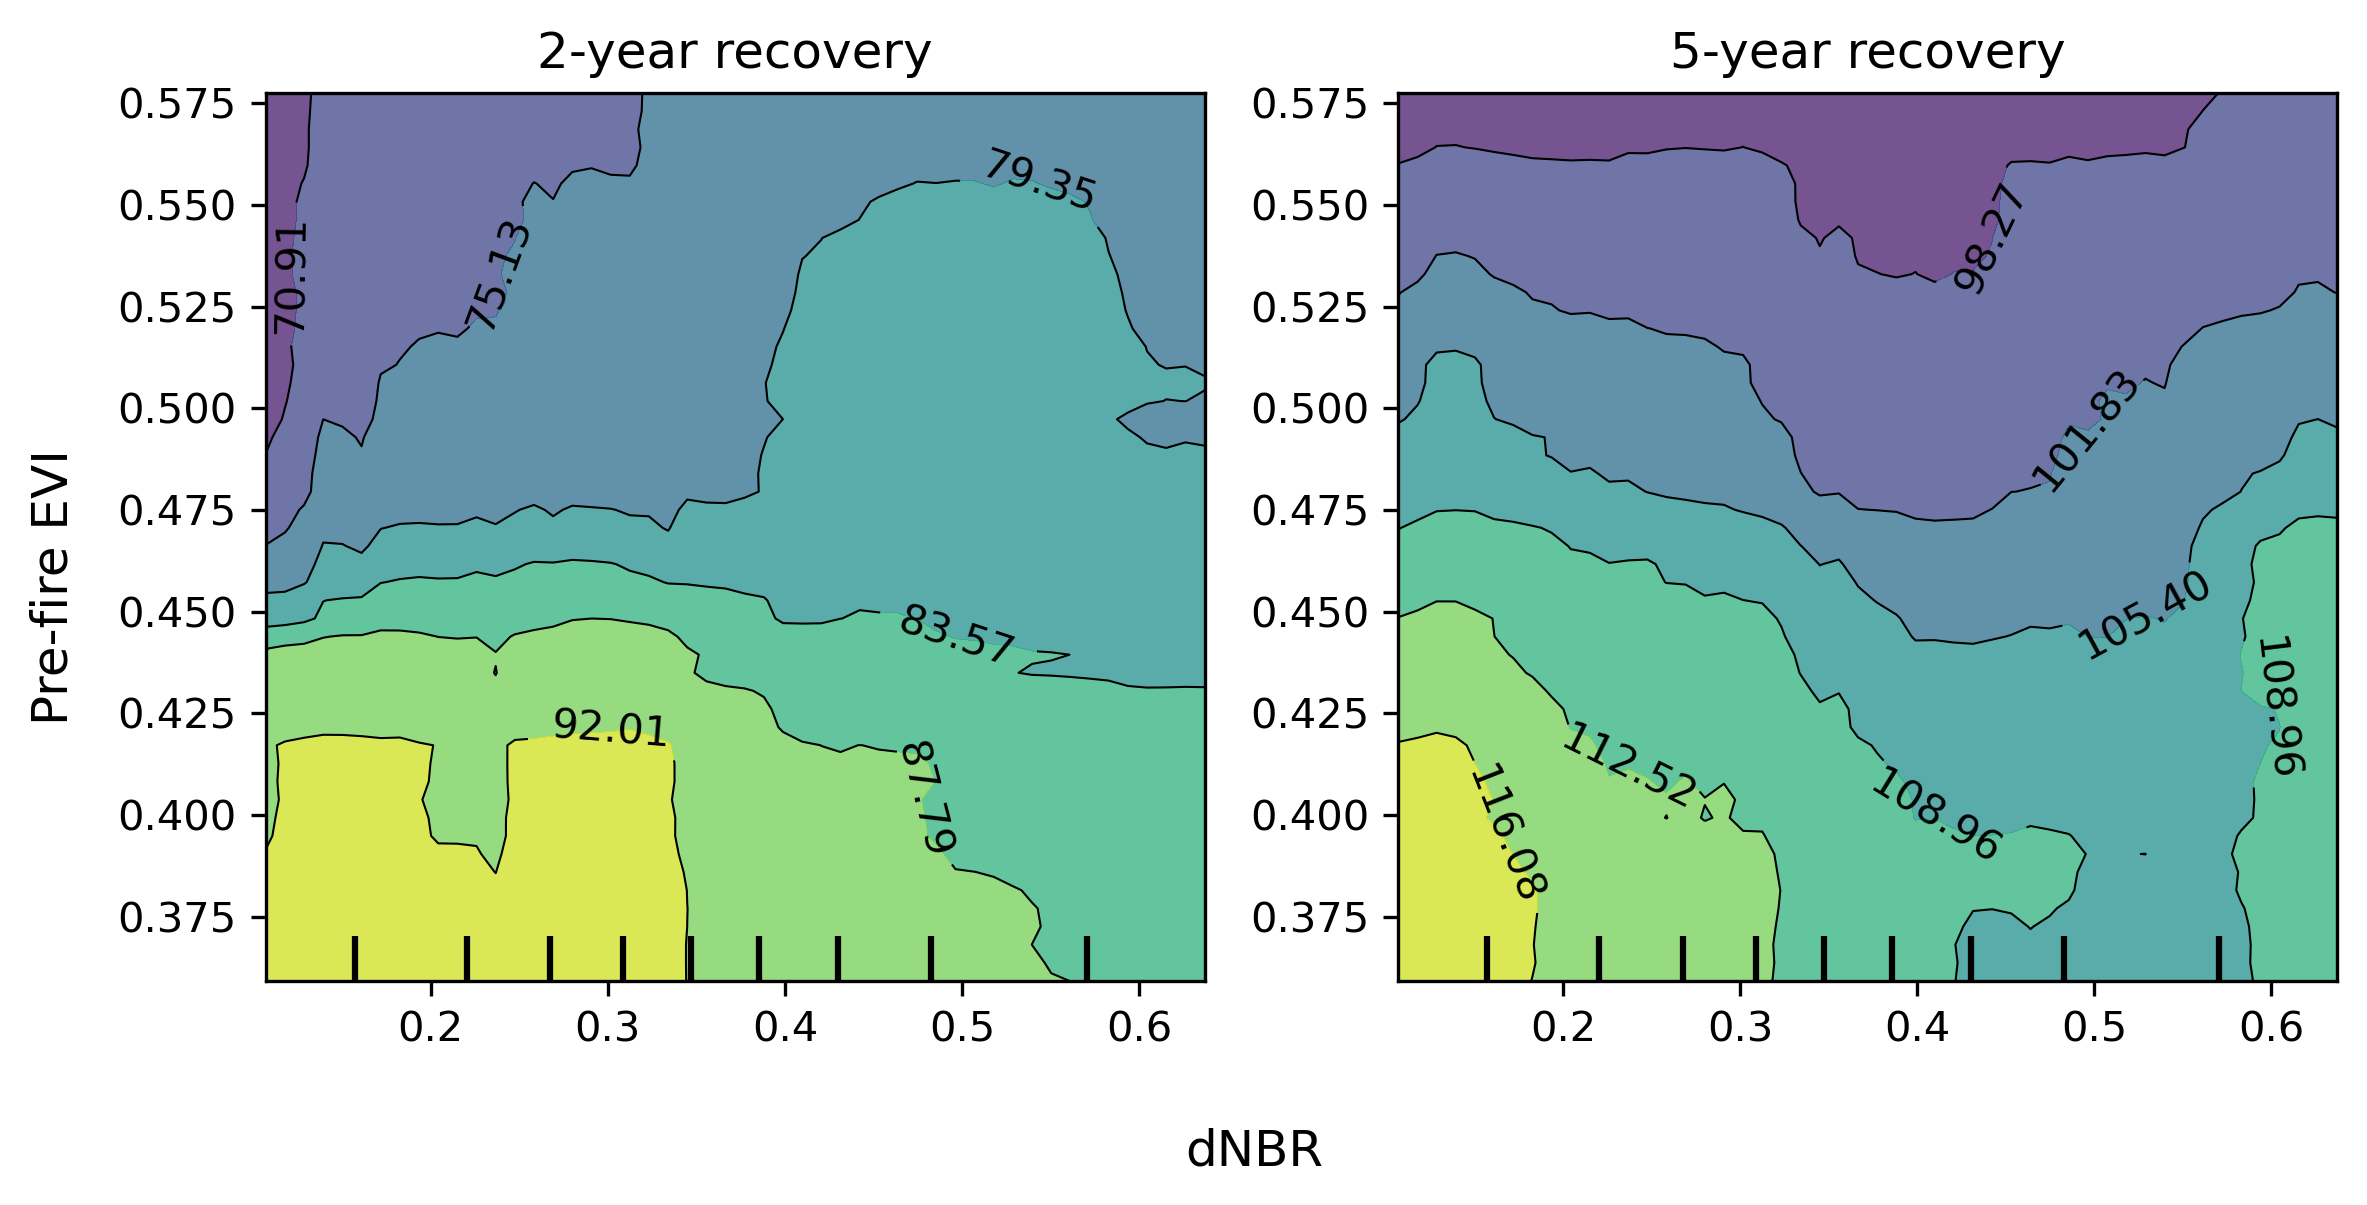
\includegraphics[width=\textwidth]{figures/pdp_2d.png}
    \caption{2-dimensional partial dependence plot showing the interactive effect of dNBR and pre-fire EVI on predicted recovery rates. Lighter colors indicate higher predicted recovery.}
    \label{fig:pdp_2d}
\end{figure}


\chapter{Discussion}


\section{Variable importance}

%Aridity
Aridity was ranked as the most influential variable on vegetation recovery over the five-year study period, and the third most influential variable over the two-year study period. Other papers, such as \textcite{zahura_impact_2024} and \textcite{qiu_quantifying_2021}, further divided post-climate conditions into precipitation and temperature, ranking them equally high in importance even in different climatic conditions in other regions of the world.
We found that recovery was higher with a high aridity index, indicating increased humidity. This aligns with expectations, as tropical peatlands function best with high moisture content. However, we were surprised to find that recovery was even better at the lower limit of aridity. The narrow range of the aridity index makes it unclear whether it can capture meaningful changes since all of the calculated values, ranging from 1.7 to 1.95, indicate a humid environment. Therefore, it is surprising that the graphs in Fig. \ref{fig:pdp_2y} and \ref{fig:pdp_5y} do not follow a linear trend. Perhaps the model has identified independent patterns that we are unable to interpret.

%Distance to drainage canals
The distance to the drainage canals, which was ranked first in importance in the short-term study period and second in importance in the longer-term study period, could not be found in another study that used a random forest model. This could be explained by the fact that the groundwater level, which was indirectly estimated by distance to drainage canals, plays a major role in tropical peatlands but possibly a minor role in other ecosystems when it comes to vegetation recovery after a wildfire. An unexpected result was that the recovery rate increased with decreasing distance to the drainage canals. This unexpected pattern may reflect restoration intervention implemented along canals network rather than a purely biophysical effect.
In Kalimantan, such interventions have been carried out at large scale by the Peatland and Mangrove Restoration Agency (BRGM), a key institution for Indonesia's peatland restoration. The agency was established after the 2015 fire crisis by Presidential Regulation (PerPres No. 1/2016) and focuses on the 3R approach: rewetting, revegetation, and revitalisation of livelihoods, targeting 2.49 Mha of degraded peatlands (\cite{giesen_roles_2023}). One of BRGM’s rewetting approaches is canal blocking, which involves constructing dams to block existing drainage canals, thereby reducing water loss and raising the water table (\cite{fleming_community_2024}). Because canal blocking is implemented directly on existing canals, areas closer to canals are more likely to have received rewetting interventions, which could help explain the higher recovery observed near drainage canals. This interpretation is supported by \cite{hooijer_benefits_2024}, who reported that fully blocked canals were rapidly overgrown with aquatic vegetation.

%Pre-fire EVI
The pre-fire EVI was ranked second in the first study period and fourth in the second, which aligns with the findings of \textcite{joao_indicator-based_2018}, who also ranked the pre-fire conditions in their Portuguese ecosystem as the second most important. Our results showed that vegetation recovered better when the EVI was smaller before the fire. Since we compared vegetation coverage after two and five years with coverage before the fire, it makes sense that lower coverage levels were reached faster than higher ones.

%Human footprint
The fourth most influential variable on vegetation recovery in the short-term study period and third in the longer-term study period was the human footprint. We decided to use it because humans are the most significant factor in long-term changes to this ecosystem. They start most fires to build plantations on the burnt land afterwards.
The recovery shows a clear improvement with increasing human impact, which could be correlated with the findings of \textcite{xu_global_2024}. Their global random forest study revealed that recovery time decreased in landscapes with a human footprint index below 7 and increased with higher values. In our results, we observed a similar substantial increase in vegetation recovery, but we did not detect a decrease above that value. As previously mentioned, a higher human footprint does not necessarily indicate negative environmental impacts. In Kalimantan, it may also capture the presence of restoration activities such as rewetting and revegetation programs.

%dNBR
The dNBR was classified as the fifth most important factor influencing vegetation recovery. However, the ranking varies greatly between different papers. While \textcite{joao_indicator-based_2018} calculated the highest importance for their "fire traits" variable in their Portuguese study area, \textcite{zahura_impact_2024} ranked burn severity as their least important variable in the northwestern US.
The effect of burn severity on recovery in our study is best interpreted in its interaction with pre-fire EVI (Fig. \ref{fig:pdp_2d}). Highest recovery rates were observed for pixels with low burn severity and low pre-fire EVI, suggesting a low absolute loss of biomass, which would recover quickly post-fire. Unexpectedly, at high pre-fire EVI, higher short-term recovery rates were predicted for higher dNBR values. High burn severity causing increased recovery has been observed in other studies, for example by \textcite{qiu_higher_2023} in Californian vegetation or by \textcite{hao_long-term_2022} in forests in China, although not specifically in peatlands yet. In those studies, increased recovery after more severe fires was linked to the rapid growth of early succession within the first one or two years after the disturbance. This pattern might also explain our observations, especially considering that in the longer-term, when this early successional vegetation has been replaced, recovery rates were equally poor at high pre-fire EVI regardless of burn severity.

%distance to nearest forest
For the two-year study period, the variable regarding distance to the nearest intact forest was classified as the second-to-last important factor influencing vegetation recovery. For the five-year study period, it was classified as the sixth most important factor. No other paper was found that included this factor in their random forest study.
Surprisingly, changes in the distance to the nearest forest had a minimal or nonexistent effect on the recovery of the vegetation. This explains the low importance in the RF model. One possible explanation for this finding is the creation of plantations on burned ground, where plants are sown simultaneously, resulting in uniform growth independent of the distance to the nearest forest.

%Elevation
Elevation was ranked as the sixth and seventh most important factor, respectively, for the two study periods. Other papers also used this factor in random forest models, where it was usually classified as equally or more important. For example, \textcite{joao_indicator-based_2018} ranked it as their third most important factor. Their study was conducted in a relatively mountainous region of Portugal that includes the Serra da Estrela mountain range. However, our study was conducted mainly in the flat coastal regions of Kalimantan, so it is difficult to compare the two studies in this context.
Different elevations showed little to no effect on the development of vegetation recovery, except for very small values that seemed to have a negative effect. This trend was particularly noticeable in the diagram of the five-year study period. This could again be explained by the creation of plantations, which are preferably started at low elevations (\cite{harris_projections_2010}).

%Fire history
Fire history was the lowest rank determinant of EVI-based vegetation recovery in both study periods of the analysis. This finding was corroborated by \textcite{joao_indicator-based_2018}, who obtained similar results. Changes in fire history values had little to no influence on vegetation recovery.
However, other studies suggest that fire history may still play an important ecological role in species composition as opposed to vegetation recovery patterns.
For example, a PCA-based analysis conducted by \textcite{giesen_roles_2023} in 2023 found that fire history strongly influences the species composition of regenerated woody pioneer vegetation in tropical peatlands. The study reported that species such as \textit{Melaleuca cajuputi} were associated with areas experiencing more than four fire events, whereas \textit{Melicope lunu-ankenda} tended to occur in areas with only one or two fire events.
This suggests that while fire history may not influence vegetation recovery patterns captured by the EVI, it may play a role in determining the species composition of regenerating peatland forests.


 \section{Random forest performance}

The Random Forest models showed moderate performance for both recovery periods. The slightly higher $R^2$ and lower RMSE in the 2-year model suggest that the selected predictors have a stronger influence on early recovery. In contrast, for longer-term recovery (5 years), additional factors beyond those included in our model may become more important. One possible explanation for the moderate model performance is that, in tropical peatlands, vegetation recovery is closely related to local hydrological conditions, such as water table depth ({\cite{hooijer_benefits_2024}}; {\cite{giesen_roles_2023}}; {\cite{ismail_recent_2023}}). However, this variable is not directly observed in our model, instead approximated using distance to drainage canals. In addition, some predictors (fire history and aridity) are only available at relatively coarse spatial resolution (approximately 1 km). This may not capture small-scale variation, thereby limiting the model performance.

Our short-term accuracy is within the range of {\cite{joao_indicator-based_2018}} that reported a $R^2$ of 0.52 for their short-term recovery (Half Recovery Time), although their study was conducted in a Mediterranean ecosystem in northern Portugal. By contrast, studies reporting higher random forest performance, such as \textcite{bright_examining_2019}, \textcite{qiu_quantifying_2021}, and \textcite{zahura_impact_2024} are not directly comparable to our results because they were conducted in non-peatland and non-tropical ecosystems. The relative importance of vegetation recovery varies among ecosystems, meaning that predictors identified as influential in other studies may not have the same role in tropical peat forests, and vice versa. Persistent cloud cover and haze in tropical regions can also increase noise in optical remote-sensing products, making vegetation recovery more difficult to predict.


\section{EVI and other vegetation recovery metrics}

Previous studies have commonly used the EVI as a proxy for vegetation recovery post-fire across a range of ecosystems, including tropical peatlands (\cite{perez-cabello_remote_2021}). Although EVI is a useful and efficient indicator for assessing vegetation dynamics it is important to acknowledge its limitations. Like other optical indices such as the Normalized Difference Vegetation Index (NDVI) and the Normalized Burn Ratio (NBR), EVI primarily reflects canopy greenness derived from spectral reflectance (\cite{bousquet_monitoring_2022}). A major limitation of optical vegetation indices is their inability to differentiate between plant species (\cite{perez-cabello_remote_2021}). This limitation is particularly relevant in tropical peatlands, where early successional vegetation often dominates post-disturbance landscapes. (\cite{blackham_natural_2014}).

In these environments, pioneer species such as shrubs, grasses, and ferns frequently colonize burned or degraded peatlands and can generate strong EVI signals due to their rapid growth and dense green cover (\cite{bousquet_monitoring_2022}), which could explain the pixels that show 100\% recovery within 2 years in our outcome variable (EVI).
However, these species are not typically characteristic of mature peat swamp forests. For example, studies have shown that pioneer species may dominate degraded peatlands and can even inhibit the regrowth of woody vegetation (\cite{blackham_natural_2014}). Consequently, this is a main justification for why recovery rates exceeding 100\% may occur within two years of fire; fast-growing pioneer species can rapidly exceed pre-fire greenness levels without representing actual forest recovery.

Moreover, methods that capture vegetation structure or species composition, such as LiDAR or field surveys, provide vertical structure information but are often costly and computationally intensive (\cite{perez-cabello_remote_2021}).
This study uses EVI, which is an efficient metric that indicates vegetation greenness, allowing monitoring over time (\cite{perez-cabello_remote_2021}).

It is worth mentioning that microwave-based remote sensing may better capture woody vegetation than optical indices. In 2022, \textcite{bousquet_monitoring_2022} performed and compared different multi-wavelengh satellite data around the world. A main finding was that L-band and C-band sensors detect vegetation water content and biomass, making them potentially more suitable for monitoring forest structure and post-fire recovery. L-band Vegetation Optical Depth (L-VOD) in particular has shown stronger sensitivity to woody biomass recovery than optical approaches (\cite{bousquet_monitoring_2022}).
Nevertheless, their key limitation is spatial resolution. Global L-band datasets from SMOS and SMAP (2015–2021) are available but operate at 9–25 km, leading to a coarser resolution. (\cite{entekhabi_soil_2010}, \cite{kerr_smos_2010}).


\section{Limitations}

A few additional limitations need to be considered when evaluating our results and their interpretation.

% As previously mentioned, peatland wildfires consist of two parts: flaming above ground and smoldering underground. For this study, which used remote sensing, we focused on the flaming, which is easier to detect from space. However, smoldering is an essential and even more damaging process that influences vegetation recovery. Future studies could therefore focus on this aspect to achieve more precise results.

Regarding the selection of predictor variables, we had to make some simplifications and most likely did not capture all ecologically relevant processes. For example, since no data was available for the water table, it was estimated based on the distance to drainage channels. However, this dataset most likely did not contain all drainage channels because they were unknown or constructed later.

Another major limitation is that human intervention, such as restoration programs, was not considered when selecting the study area, primarily due to the absence of spatially explicit data. Thus, some pixels might have experienced human-assisted recovery. For example, in 2017, 19,670 seedlings of local tree species were planted as part of ecosystem restoration programs {\cite{lestari_understanding_2022}}. In the same year, 84 box dams were constructed as well as 212 compacted peat dams (\cite{giesen_roles_2023}), modifying local hydrological conditions.

Furthermore, we employed random forest regression, which is a commonly used method in research on post-fire vegetation recovery. While it usually has moderate to high predictive power, the interpretation of variable effects can be challenging. In our study, this limitation was most clearly illustrated by the aridity index, which was ranked as one of the most important variables but had a highly non-linear pattern in the partial dependence plot (Fig. \ref{fig:pdp_2y} and \ref{fig:pdp_5y}) that we could not explain ecologically. In addition, RFR cannot extrapolate beyond the value range it was trained on. A number of our predictors had very skewed distributions or limited value ranges (see Fig. \ref{fig:hist_pred1} and \ref{fig:hist_pred2}), which might have obscured truly ecologically meaningful relationships between factors and recovery rates. These limitations underscore the importance of domain knowledge to distinguish possible causal relationships between predictors and recovery rates from purely statistical or spatial patterns learned by a model.

Lastly, due to the scope of the project, our analysis was limited to the state of recovery at two specific points in time -- two years (2017) and five years (2020) after the fires -- which we investigated using separate models. This study design meant that we did not account for yearly differences, such as particular climatological conditions, that might have affected vegetation, and thereby recovery rates, overall. For a more comprehensive analysis, a methodology such as the one employed by \textcite{zahura_impact_2024} could be transferred to tropical forests. In this study, the authors used RF to predict the incremental recovery of vegetation in burned areas in the Pacific Northwest. The year-by-year EVI changes per pixel were treated as separate observations to train the same model, with the number of years since the fire as an additional predictor. This approach yielded exceptionally high R$^2$ values between 0.89 and 0.945 for testing.


\chapter{Conclusion}

% do we want to say we trained two models? or shall we just refere as one
%EVI shall we say is common practice in the conclusion, i think is already said before in the discussion.
% should we mention something abiout floods before?
%The Enhanced Vegetation Index (EVI) served as the recovery measure, acknowledging its inherent limitation to vegetation greenness and its inability to capture structural or species-level recovery.

This study identified eight variables influencing short-term (2-year) and longer-term (5-year) vegetation recovery in tropical peatlands in Kalimantan following the 2015 fires. These variables, derived primarily from satellite imagery and complementary datasets. Then, a random forest model was trained to predict the recovery metric: the Enhanced Vegetation Index (EVI).

The RF model revealed that no single variable dominated the recovery outcome; however, five variables exceeded 10\% relative importance. The three most influential variables were aridity index, distance to drainage canals, and pre-fire EVI. These findings suggest that post-fire recovery is controlled by a combination of climatic, hydrological, and antecedent conditions rather than any single factor.

Post-fire vegetation recovery studies in tropical peatlands have employed inconsistent metrics and no standardized assessment approach exists. To our knowledge, this study presents the first predictive model of post-fire vegetation recovery in tropical peat forests, limiting direct comparison with similar studies.

The study's findings are limited by the absence of field-validated measurements, subsurface peat combustion characterization, and water table data. The coarse spatial resolution and potential overlooked variables may fail to capture the full complexity of vegetation. Future work should address these gaps while analyzing inter-annual and seasonal variability as well as non-optical vegetation metrics. Given tropical peatlands' critical role in global carbon storage and their vulnerability to repeated fire disturbance, enhanced monitoring efforts are essential to inform targeted interventions for vegetation recovery.

\chapter*{Code availability}

The Jupyter Notebooks and the Google Earth Engine script used to conduct the analysis, as well as the TeX document to render this report are available on GitHub: https://github.com/ninorp55/tropical-peat-post-fire-vegetation-recovery

\begingroup
\renewcommand{\cleardoublepage}{}
\renewcommand{\clearpage}{}
\chapter*{Documentation of AI use}
\endgroup

We used tools based on Artificial Intelligence (AI) as a support in different aspects of the research process.

\textbf{Conceptualization and writing}

- Consensus AI (https://consensus.app/) and Perplexity AI (https://www.perplexity.ai/) to search for literature

- ChatGPT 5.3 (https://chatgpt.com/) and DeepL AI https://www.deepl.com/)to improve grammar, clarity and flow of writing

\textbf{Technical implementation}

ChatGPT 5.3 (https://chatgpt.com/) and Claude Sonnet 4.6 (https://claude.ai/new) used to assist with:

- development of GEE scripts for data extraction

- debugging code and increasing computational efficiency

- creating and modifying code for figures

- implementing spatial operations such as rasterization and distance computation in Python



% bibliography
\printbibliography


\chapter*{Appendix: Additional visualizations} \label{appendix}

% reset figure counter
\renewcommand{\thefigure}{A\arabic{figure}}
\setcounter{figure}{0}

\begin{figure}[H]
    \centering
    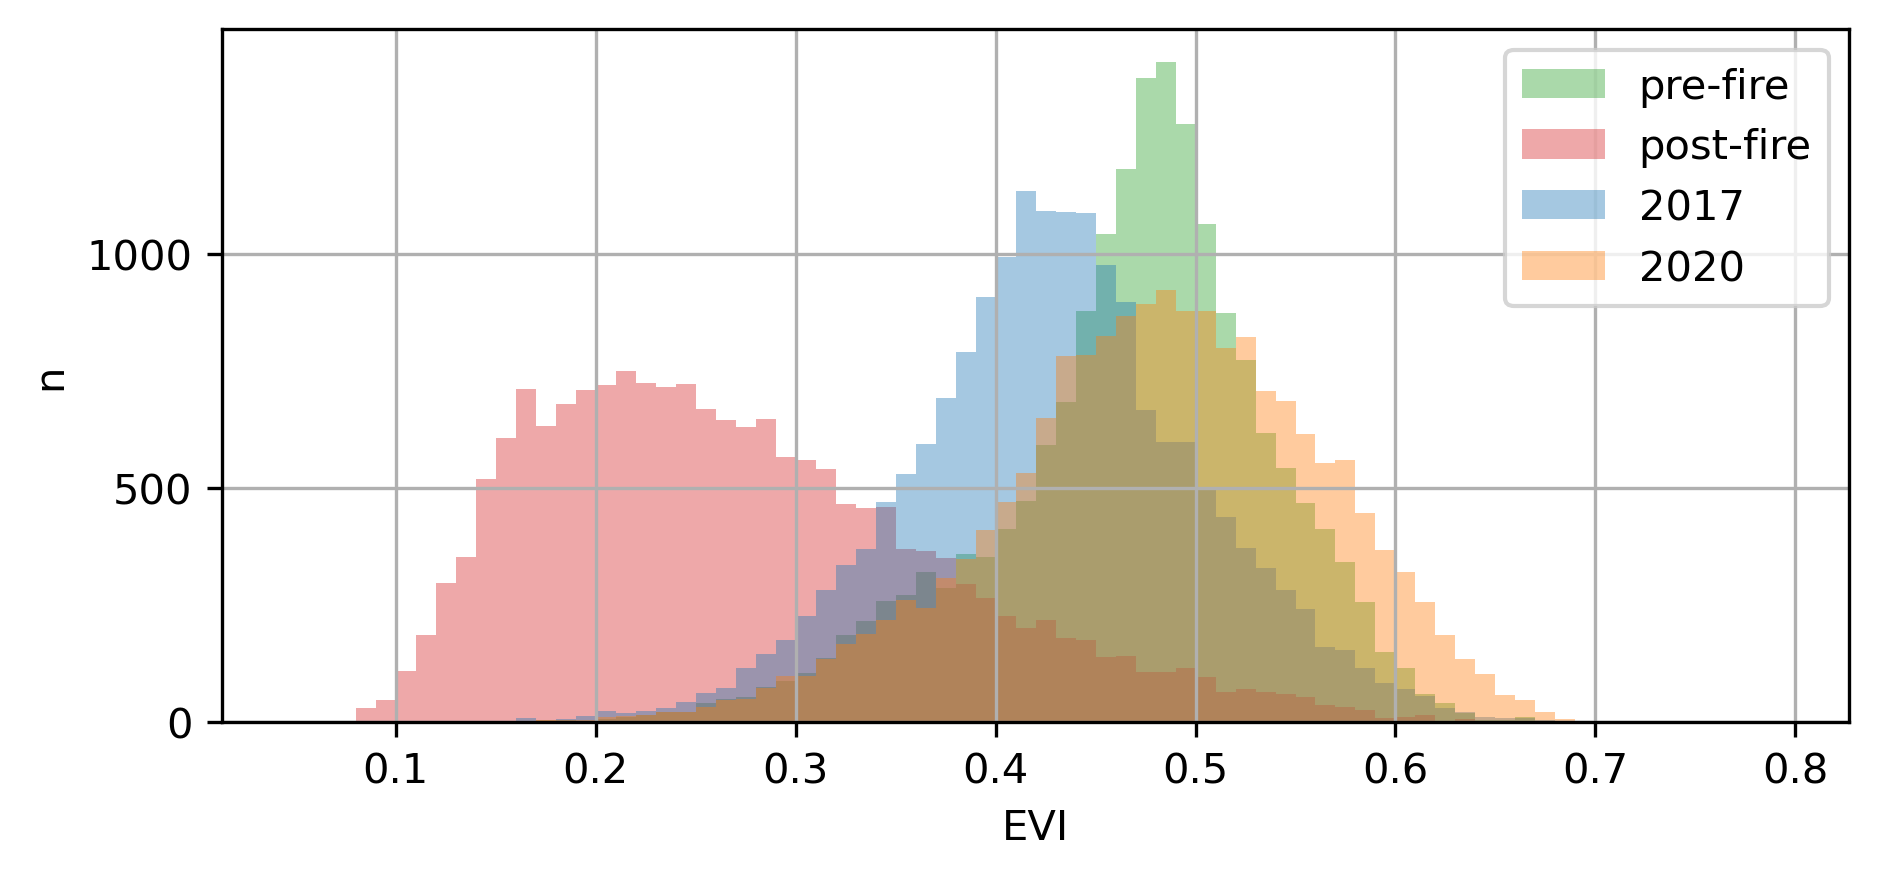
\includegraphics[width=\textwidth]{figures/hist_evi.png}
    \caption{Distribution of EVI values in the study area at different points in time. Pre-fire EVI is the 5-year median up until July 2015. Post-fire EVI is the 3-month median from November 2015 to January 2016. 2017 and 2020 are yearly medians. n refers to the number of pixels in the study area.}
    \label{fig:hist_evi}
\end{figure}

\begin{figure}[H]
    \centering
    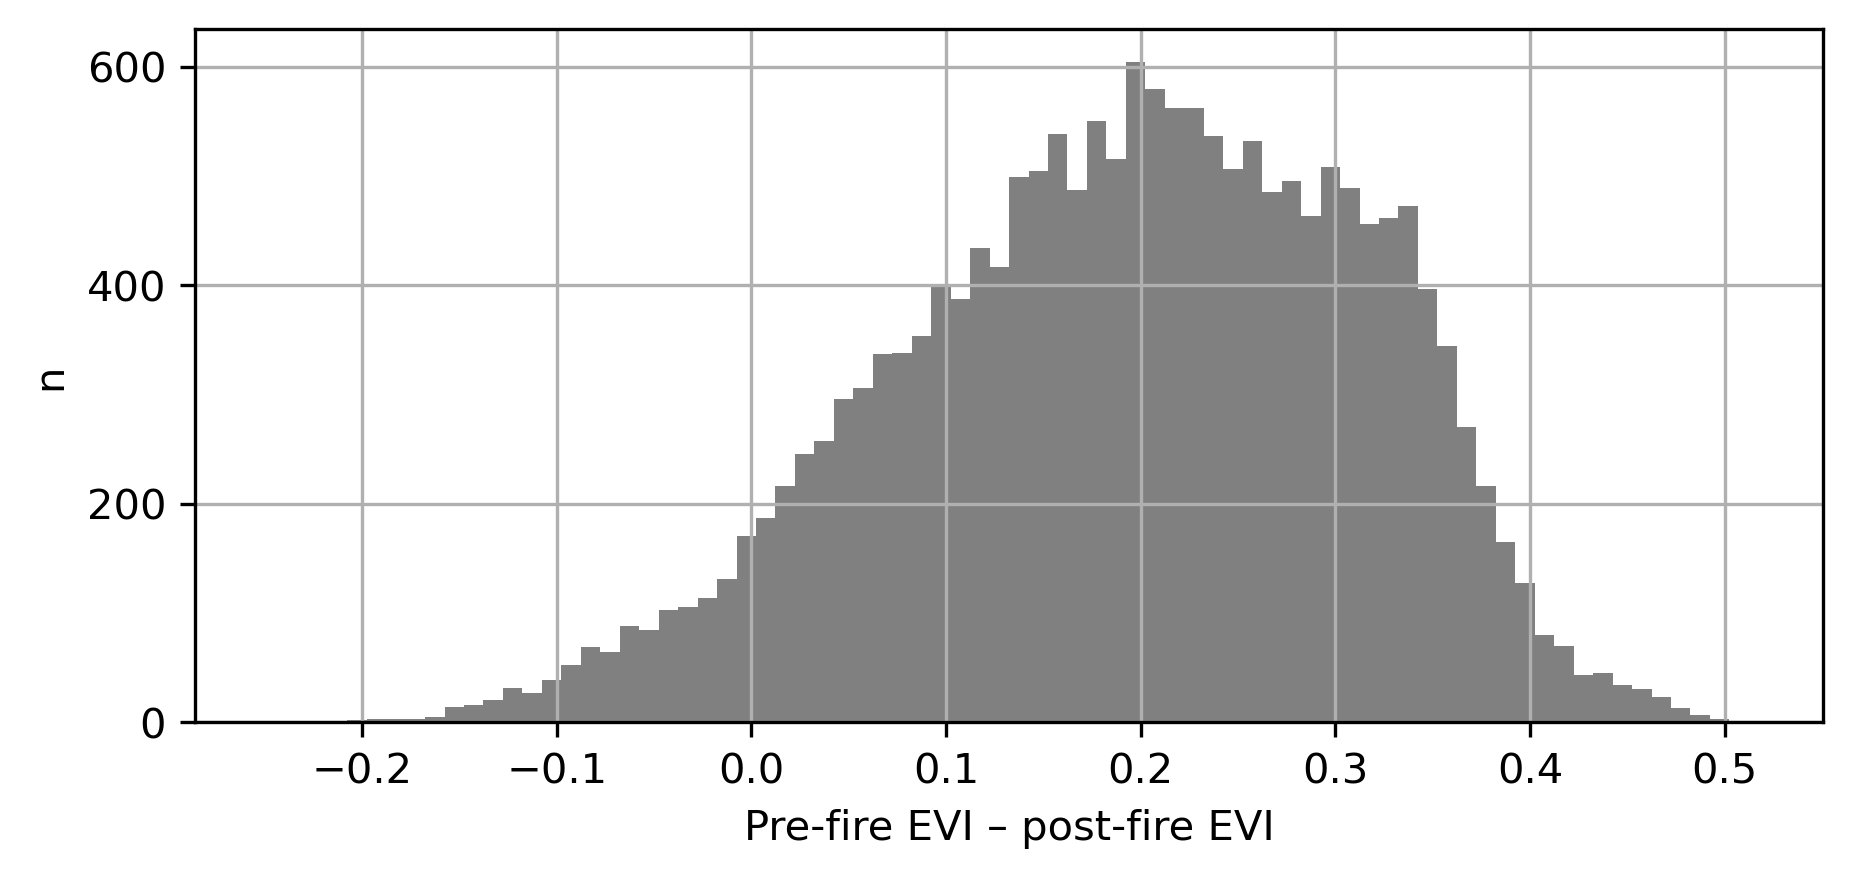
\includegraphics[width=\textwidth]{figures/hist_evi_diff.png}
    \caption{Distribution of differences between pre- and post-fire EVI. Positive values indicate reduction of EVI. n refers to the number of pixels in the study area. Pixels with values below 0.1 were excluded from the analysis since they do not represent fire-related vegetation loss.}
    \label{fig:hist_evi_diff}
\end{figure}

\begin{figure}[H]
    \centering
    
\includegraphics[width=\textwidth]{histogram_panel_pt1.png}
    \caption{Distribution of (a) Human Footprint Index, (b) Aridity Index, (c) Fire History, and (d) Elevation. Human footprint, fire history, and elevation are right-skewed. Aridity is more symmetrically distributed around the center. Each panel shows mean ± standard deviation}
    \label{fig:hist_pred1}
\end{figure}

\begin{figure}[H]
    \centering
    
\includegraphics[width=\textwidth]{histogram_panel_pt2.png}
    \caption{Distribution of (e) Distance to Drainage, (f) Distance to Forest, (g) Pre-fire EVI, and (h) Difference Normalized Burn Ratio (dNBR). Distance variables are strongly right-skewed. Pre-fire EVI and dNBR show approximately bell-shaped distributions. Each panel shows mean ± standard deviation.}
    \label{fig:hist_pred2}
\end{figure}

\end{document}
